\documentclass[12pt,a4paper]{report}
\usepackage{graphicx}
\usepackage[letterpaper, portrait, left=2cm, right=2cm, top=2.5cm, bottom=2.5cm]{geometry}
\usepackage[labelfont=bf, hypcap=false]{caption}
\usepackage{subcaption}
\usepackage{placeins}
\usepackage{float}
\usepackage{url}
\usepackage[dvipsnames, table]{xcolor}
\usepackage{sectsty}
\usepackage[square,numbers]{natbib}
\usepackage[Conny]{fncychap}
\usepackage{lipsum}
\usepackage[toc,page]{appendix}
\usepackage{hyperref}
\usepackage{multirow}
\usepackage{mathrsfs,amsmath,amssymb}
\usepackage{esvect}
\usepackage{physics}
\usepackage[english]{babel}
\usepackage{cancel}
\usepackage{listings}
\usepackage{anyfontsize}
\newcommand{\Lagr}{\mathcal{L}}
\graphicspath{{images/}}
\usepackage{collcell}
\usepackage{hhline}
\usepackage{pgf}
\usepackage{colortbl}
\usepackage{tabu}
\usepackage[T1]{fontenc}
\usepackage[latin9,utf8]{inputenc}
\usepackage{pifont}
\usepackage{animate}
\usepackage{fancyhdr}
\usepackage{booktabs}
\usepackage{lipsum}% just to generate text for the example


\newcommand\items{3}
\newcommand*\rot{\rotatebox{90}}


\ChTitleVar{\centering\Huge\scshape\color{RoyalBlue}}
\ChNameVar{\centering\Huge\fontfamily{pbk}\selectfont\scshape\color{RoyalBlue}}

\makeatletter
\renewcommand{\DOCH}{%
	\color{ForestGreen}\mghrulefill{3\RW}\par\nobreak
	\vskip -0.5\baselineskip
	\mghrulefill{\RW}\par\nobreak
	\CNV\FmN{\@chapapp}\space \CNoV\thechapter
	\par\nobreak
	\vskip -0.5\baselineskip
}
\makeatother

\begin{document}
\begin{titlepage}


				\centering

				%\vspace*{\stretch{1}}
				{\Large\fontfamily{pbk}\selectfont Signal and background discrimination in the top squark production with   $\text{1\textit{l}} + \cancel{\it{E}}_{T} $ final states using Machine Learning and Data Visualisation \par}
				\vspace{1.0cm}
			%$ \Tilde{t}\Tilde{t^*} \rightarrow t \Bar{t} \Tilde{\chi^0_1}\Tilde{\chi^0_1} \rightarrow b\Bar{b}l^{+}jj\cancel{\it{E}}_{T} $	     
			    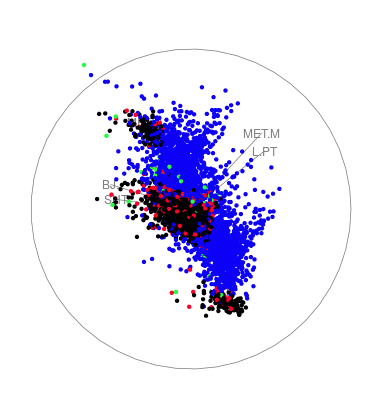
\includegraphics[width=0.6\textwidth]{title.png}\par\vspace{1cm}
				%\vspace{1cm}
				{\Large\itshape Kenji Sato Macfarlane\\}
				\vfill
				Supervised by:\par
				Dr. Ursula Laa \par 
				Co-supervised by:\par
				Professor German Valencia \\
				
				\vfill
				
\includegraphics[width=0.175\textwidth]{monashlogo.png}\par\vspace{0.5cm}
				
				{\large \today\par}

\end{titlepage}
%-------------------------------------------------------------------------%
%\thispagestyle{empty}
%\begin{center}
%    \vspace*{\stretch{1}}
%    \textit{I would like to dedicate this thesis to my loving family and parents, especially to my father who is sadly no longer with us.}
%    \vspace*{\stretch{1}}
%\end{center}
%\clearpage

\pagenumbering{roman}
\setcounter{page}{1}
\begin{center}
    \vspace*{\stretch{1}}
    \section*{\centering \Huge Acknowledgement}
    I would like to thank my supervisors Ursula and German for taking me on as their student and giving me guidance throughout the year.
    \vspace*{\stretch{1}}
\end{center}
\clearpage


%\begin{center}
%    \vspace*{\stretch{1}}
%    \section*{\centering \Huge Abstract}
%    \noindent 
%    \vspace*{\stretch{1}}
%\end{center}
\begin{abstract}
    \noindent The Minimal Supersymmetric Standard Model serves as an extension to the Standard Model in which we observe the simplified model for the top squark decaying into a topquark-neutralino pair: $pp \rightarrow \Tilde{t}\Tilde{t^*} \rightarrow t \Bar{t} \Tilde{\chi^0_1}\Tilde{\chi^0_1} \rightarrow b\Bar{b}jjl\cancel{\it{E}}_{T}$. We simulated the process at four different mass parameters for the top squark and neutralino masses and performed statistical analysis including machine learning, in which we observed low AMS values of up to 2.8. Visualising the data in a guided tour, we observe that the $\cancel{\it{E}}_{T}$, the $\phi$ component of the $\cancel{\it{E}}_{T}$ and charged lepton, the $p_T$ of the lepton and the hadronic energy $H_T$ had strong contributions to the result.
\end{abstract}
\clearpage

%-------------------------------------------------------------------------%
\makeatletter
\renewcommand\tableofcontents{%
    \if@twocolumn
      \@restonecoltrue\onecolumn
    \else
      \@restonecolfalse
    \fi
   \newgeometry{top=1.8cm, bottom=1.8cm, left=2cm, right=2cm}
    \chapter*{\contentsname
        \@mkboth{%
           \MakeUppercase\contentsname}{\MakeUppercase\contentsname}}%
    \@starttoc{toc}%
    \if@restonecol\twocolumn\fi
    \restoregeometry
    }
\makeatother

\tableofcontents
\clearpage

%-------------------------------------------------------------------------%
\pagestyle{fancy}
\fancyhead[L]{\empty}
\fancyhead[R]{\footnotesize
  \begin{tabular}[b]{@{}r@{}}
    \nouppercase{\leftmark}\\[3pt]
    \nouppercase{\rightmark}
  \end{tabular}%
}
\setlength{\headheight}{27pt} % check the log to be sure what this length should be
%-------------------------------------------------------------------------%

\pagenumbering{arabic}
\setcounter{page}{1}

%---------------------------------------------------------------------------%
\chapter{Introduction}
%For centuries, philosophers and physicists have delved into the idea of what constructs and drive living beings including, in the grand scale, the universe as we know it. From the development of classical mechanics by the likes of Galileo Galilei and Sir Isaac Newton in the 17th Century, to the discovery and fundamental establishment of electromagnetism in the 19th Century by the likes of Michael Faraday, André-Marie Ampère, Hans Christian Ørsted, and James Maxwell, physicists have achieved a phenomenal feet throughout modern history. These establishments became building blocks and in the 20th Century society witnessed further advancements. In particular, the foundations of the connection between quantum mechanics and particle physics were built by the likes of Emmy Noether (Noether's theorem for conservation laws), Richard Feynman (Quantum Electrodynamics and Feynman diagrams), Hideki Yukawa (Yukawa coupling). We have started to quantize nature to reach a deeper understanding, and the particle physics community established fundamental properties to matter and forces entering the 21st Century.  \\

Fast forward to July 2012, the world received the news of the discovery of the Higgs Boson through experiments at the Large Hadron Collider (LHC) \cite{chatrchyan2012observation,aad2012observation}. The discovery completed the extent of the Standard Model (SM) as we know it, where three of the fundamental forces - strong, weak and electromagnetism - are well encapsulated giving a firm ground to the three generations of fundamental particles in quarks and leptons. However, the SM itself is an incomplete theory. This stems from the fact that the other fundamental force, gravity, remains unanswered at the quantum scale and how it contributes to the elementary particles. Unifying all four forces was Albert Einstein's dream, and remains a goal for physicists of the present and future. Another reason is due to 'dark matter' not being observed directly at the elementary particle scale yet, despite accounting for roughly $25\% $ of the universe's critical density \cite{bahcall2015dark}. There are many more problems such as the hierarchy problem, the neutrino mass problem and the need for three generations of fundamental particles and so on, that could be expanded upon depending on the field of interest. \par

%This stems from the fact that the observed mass of $ m_H \approx 125\text{GeV} $ of the Higgs Boson is 'too light'. This is known as the gauge hierarchy problem \cite{martin1997supersymmetry}, where the squared Higgs mass ($ m^2_T $) requires quantum corrections from invisible (virtual) particles and fields to reach the minimum value. \par

A proposed solution to these issues is Supersymmetry (SUSY), where so-called super-partners of the SM particles are introduced. These super-partners are initially theorized to be of equal mass to the SM counterparts. However, the experimental endeavor for such particles disproves that, leading us to the understanding that they must be extremely heavy. Furthermore, SUSY predicts a symmetry-breaking in a way that allows the observed Higgs mass to be valid. It is also predicted that, electromagnetism, strong, and the weak force would still hold in high energy scales that correspond to the early universe just after the Big Bang. Quantum gravity is accounted for at the Plank scale $ M_p = (8\pi G_{\text{Newton}})^{-1/2} = 2.4 \times 10^{18} \text{GeV} $, although it is much larger than the electroweak scale \cite{martin1997supersymmetry}, hence making it a difficult task to sought out not only gravity but the super-partners as well. If SUSY turns out to be a successful model, then it signifies the high energy physics community is heading toward the right direction to formulate the Grand Unifying theory - where all four fundamental forces are united mathematically. \\

%To test the correctness of SUSY, further experiments have been conducted at the LHC in the quest to find said superparticles. This seems to be a dead-end to high energy physicists as none of the theorized phenomena nor particles from SUSY have been observed directly, despite the upgrade in the collider's energy levels. 
Since the search for phenomena beyond SM has proven to be difficult, the most obvious solution is to produce collisions at a much higher center-of-mass ($\sqrt{s}$) energy than what the LHC currently produces (13TeV). This is problematic as building a much larger facility is unavoidable if physicists were to pursue this route. Instead, the sensitivity and signal selection to SUSY can be achieved with the current resource available. With an upgrade to the High-Luminosity LHC set to be ready by 2026 \cite{apollinari2015high, apollinari2017high} which will see the collision rate of protons increased by a factor of 10, there is hope that the increased amount of data improves the sensitivity of the searches for SUSY. \\

Machine Learning comes into play here in particular for signal selection. Machine learning has made a significant impact in the past few decades not only in scientific areas but also in industry. The emergence of 'Big Data' accumulated over the years has allowed the refinement of machine learning models and increased its reliability in real-world applications. The Higgs Boson was discovered with the help of machine learning \cite{chatrchyan2012observation,aad2012observation}. High energy physics has been a frontier to employing machine learning techniques and is essentially a gold mine for data scientists. A fraction of the available data is made public partly due to its sheer size. To give a sense of how large the produced data is, CERN has a self-established network across the globe dedicated to handling the 25 petabytes (initially 15 \cite{shiers2007worldwide}) of data produced a year known as the Worldwide LHC Computing Grid (WLCG), which is said to be the largest in the world. Since $1\text{PB} = 10^6\text{GB}$, it is easy to see that this is a massive amount of data, requiring $10^5$ computers to operate through such amount at the time of proposal \cite{shiers2007worldwide} (it would be roughly $10^3$ now as a decent computer would have 1TB = 1000GB of storage space available). With the evolution of machine learning and the endless supply of data produced by the LHC, a more complete and systematic study for refinements in SM and SUSY both experimentally and theoretically.\\

The following sections will introduce some basic concepts to understand the key areas of the standard model and SUSY required for the project. Subsequent sections will introduce approaches and concepts necessary for the project, such as the methods of searching for SUSY (in particle, the Minimum Supersymmetric Standard Model i.e. MSSM), the decay channel of stops and basic concepts and research applications of machine learning algorithms.


%-------------------------------------------------------------------------%
\chapter{The Standard Model and Beyond}
\label{chap:2}
%\section{The Standard Model and Beyond}

%-------------------------------------------------------------------------%
\section{The Standard Model}
The Standard Model (SM) consists of three generations of matter as \textit{fermions} of spin-$1/2$ and three fundamental forces\footnote{Electromagnetism, the Weak force and the Strong force. gravity is not yet fully understood at the quantum scale, therefore it is not included in the SM.} including the Higgs as \textit{bosons}\footnote{The Higgs Boson is spin-0, whereas the other bosons are spin-1.}. The three fundamental forces interact with the fermionic matter through its own unique corresponding Quantum Field Theory (QFT), in which the interaction of matter with the Higgs field provides the masses to such particles as we measure to date. \\

Fermionic matter consists of \textit{leptons} and \textit{quarks}, in which Table \ref{tab:SMFerm} depicts. Each of the three generations of quarks have an up-type and a down-type quark categorized by their charges ($+2/3 \text{ or } -1/3$), and the leptons consist of charged and neutral leptons in which the neutral components are known as neutrinos. The up-type quarks are the \textit{up}, \textit{charm} and \textit{top} quarks, and the down-type quarks are the \textit{down}, \textit{strange} and \textit{bottom} quarks. These quarks, except for the top quark, exist in a bound state known as \textit{hadrons} and can never be observed directly. Hadrons are categorized into mesons or (anti-)bayons\footnote{Mesons consist of two quarks; one quark and anti-quark each. (Anti-)Baryons consist of three (anti-)quarks.} in which the proton and neutrons are a family of \cite{thomson2013modern}. The first generation of elementary particles represent the basic building blocks of the low energy Universe, and more complex interactions are mediated by the second and third generations \cite{thomson2013modern}. Furthermore, these particles differ greatly in mass where the later generations are much heavier than the first. \\

\begin{table}[htbp]
    \centering
    \begin{tabular}{||c|c|c|c||}
    \hline
    & Gen1 & Gen2 & Gen3 \\
    \hline
    \multirow{2}{1.2cm}{quarks} & $u$ & $c$ & $t$ \\
     & $d$ & $s$ & $b$ \\
    \hline
    \multirow{2}{1.2cm}{leptons} & $e$ & $\mu$ & $\tau$ \\
     & $\nu_e$ & $\nu_\mu$ & $\nu_\tau$ \\
    \hline
    \end{tabular}
    \caption{The three generation of fermionic matter in the Standard Model. From the top row, left to right, we have the up, charm, top, down, strange and bottom quarks, followed by the electron, muon and tau for the charged leptons and their associated neutrinos as neutral leptons. All fermions in this table have spin-$1/2$.}
    \label{tab:SMFerm}
\end{table}


The gauge bosons consist of four vector bosons in the form of \textit{gluons}, \textit{photons}, \textit{Z bosons} (neutrally-charged) and \textit{W bosons} (electrically charged). The photon mediates electromagnetism (QED) and the gluons mediate the strong force (QCD) where the interactions in theory relies on them being mass-less, which are already experimentally verified. The weak force is mediated by the Z and W bosons, which are massive; roughly 80 and 91GeV/c$^2$ respectively, to be precise \cite{tanabashi2018review}. The weak gauge bosons and the photon are `produced' through the Higgs mechanism and electroweak symmetry breaking. In essence, the Higgs field which is a doublet that contains a neutral and a charged component, acquires some vacuum expectation value (vev) which produces a physical Higgs and some massless Goldstone bosons. This is known as the Higgs mechanism. Through broken symmetries and mixing, the photon arises from the $B$, the $Z^0$ arises from $W^3$ and the $W^\pm$ arises from the $W^1 \pm iW^2$ components of the electroweak Lagrangian's field tensors \cite{thomson2013modern}. These terms will be relevant again when we touch on supersymmetry. \\

\begin{table}[htbp]
    \centering
    \begin{tabular}{||c|c||}
    \hline
       Gauge Bosons  & Scalar Bosons \\
     \hline
       $g$, $\gamma$ ($B$), $Z^0$ ($W^3$), $W^\pm$ & $H^0$ \\
     \hline
    \end{tabular}
    \caption{Force carriers (bosons) in the Standard Model. The gauge bosons consist of the gluon, photon, Z boson and W bosons, where the photon and Z boson originate from the $B$ and the $W^3$ components. The Higgs boson is the only known scalar in the SM with spin-0, opposed to the gauge bosons that are vector bosons and have spin-1.}
    \label{tab:SMBos}
\end{table}


%-------------------------------------------------------------------------%
\section{The top quark and its decay}
Amongst the SM particles, the top quark interests us the most as this will correspond to our background events.  The top quark has a rest mass of $m_t\approx175\text{GeV/c}^2$ (we will express mass and energy in natural units $c=1$ hereon) and an electric charge of +2/3$e$ \cite{tanabashi2018review} making it the only known elementary particle in the SM to be heavier than the Higgs boson. The theoretical predictions of top quarks and the bottom quark was established in 1973 by Kobayashi and Masakawa to explain charge-parity (CP) violation in some meson decays \cite{griffiths2008introduction, kobayashi1973cp}. Experimental evidence for the bottom quark, the generationally paired particle to the top quark, was found at Fermilab in 1977 \cite{herb1977observation}. Nearly two decades later in 1994, the top quark was discovered at the Tevatron with an energy\footnote{The Centre-of-Mass energy, denoted as $\sqrt{s}$, is a Lorentz invariant value such that $s=\Big( \sum\limits_{i=1}^2 E_i \Big)^2 - \Big( \sum\limits_{i=1}^2 \overrightarrow{p_i} \Big)^2 $. Note that $c=1$ and each $i$ represents the protons in the beam.} of $\sqrt{s}=1.8\text{TeV}$ through the process $p\Bar{p} \rightarrow t\Bar{t}$ \cite{abachi1994search, coll1994evidence, abachi1995observation}. The top quark almost always decays through the weak interaction into a bottom quark and a W boson pair. The W boson then produces a charged lepton-neutrino pair or a pair of quark-antiquark that form hadronic jets. These possible decay modes are given in Figure \ref{fig:topdecay}. \\

\begin{figure}[htbp]
    \centering
    \begin{minipage}{0.24\linewidth}
        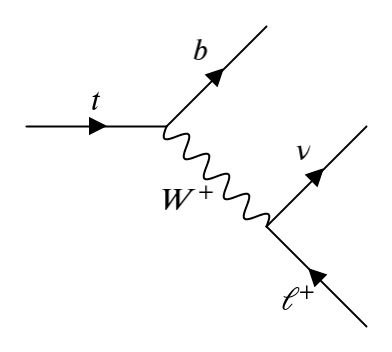
\includegraphics[width=\linewidth]{top1.png}
        \label{fig:top1}
    \end{minipage}
    \begin{minipage}{0.24\linewidth}
        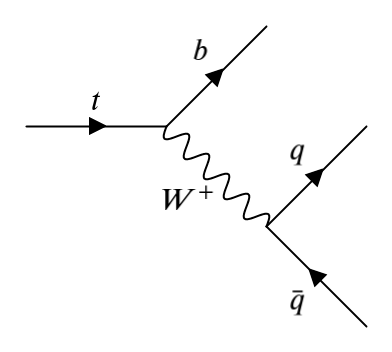
\includegraphics[width=\linewidth]{top2.png}
        \label{fig:anttop1}
    \end{minipage}
    \begin{minipage}{0.24\linewidth}
        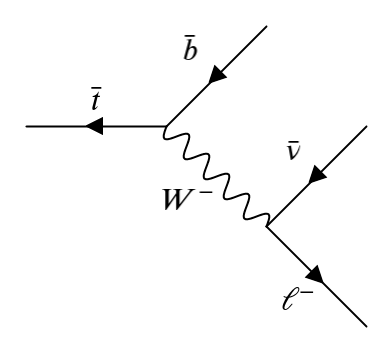
\includegraphics[width=\linewidth]{top3.png}
        \label{fig:top2}
    \end{minipage}
    \begin{minipage}{0.24\linewidth}
        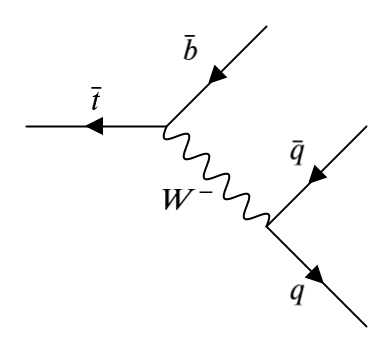
\includegraphics[width=\linewidth]{top4.png}
        \label{fig:anttop2}
    \end{minipage}
    \caption{Feynman diagrams of possible (anti-)top decays. From left to right, we see the top decay with leptonic final states, top decay with hadronic final states, anti-top decay with leptonic final states and anti-top decay with hadronic final states.}
    \label{fig:topdecay}
\end{figure}

%-------------------------------------------------------------------------%
\section{The Minimal Supersymmetric Standard Model}
The Minimal Supersymmetric Standard Model (MSSM) serves as an extension to the SM such that the particle content is duplicated once, thus keeping extra particles introduced to its minimum. Due to the symmetry groups of the SM being contained in the MSSM, any supersymmetric transformation would yield the same quantum numbers as that of the SM \cite{aitchison2007supersymmetry}. The fermions and bosons in the SM shown in Tables \ref{tab:SMFerm} and \ref{tab:SMBos}  have \textit{superpartners}; the supersymmetric counterparts to each particle in the SM as seen in Tables \ref{tab:SUSYspart} and \ref{tab:SUSYinos}. By convention the SM particles and their superpartners are distinguished by a tilde. \\

The MSSM relies on an extended theory to the SM known as the Two-Higgs-doublt model (2HDM), in which the SM Higgs consists of the up-type Higgs ($H_u$) and the down-type Higgs ($H_d$) that contain both neutral and charged components. The SM currently only has one Higgs doublet, giving rise to four degrees of freedom that produce the Higgs boson and the gauge bosons in the SM. In the 2HDM, the number of degrees of freedom doubles to eight, leading to 5 scalar components including the physical Higgs boson. In the MSSM, the superpartners of the Higgs, the Higgsinos, are the superpartners to the 2HDM, hence the two components in Table \ref{tab:SUSYinos}. \\

The superpartners to the SM particles are called \textit{squarks}, \textit{sleptons} and \textit{sneutrinos} whereas the superpartners to the bosons in the SM end with an ``-ino" e.g. \textit{gaugino}. The `symmetry' depicted in supersymmetry is the symmetry between fermions and bosons. This means that the fermions in the SM are bosons in the MSSM and vice versa \cite{martin1997supersymmetry}. Tables \ref{tab:SUSYspart} and \ref{tab:SUSYinos} illustrate that the number of new particles introduced is kept to a \textit{minimum} \cite{aitchison2007supersymmetry}. There is one problem, however. This symmetry we see in Tables \ref{tab:SMFerm}-\ref{tab:SUSYinos} would require that these MSSM particles have the same masses as their SM counterparts. We know this not to be true simply from such particles not being observed in collider experiments thus far. The symmetry must be broken at some high energy scale in an unknown way, allowing these particles to acquire much heavier masses to their SM counterparts that is unobservable with current collider experiments. \\

\begin{table}[htbp]
    \centering
    \begin{tabular}{||c|c|c|c||}
    \hline
    & Gen1 & Gen2 & Gen3 \\
    \hline
    & \\[-2.7ex]
    \multirow{2}{1.4cm}{squarks} & $\Tilde{u}$ & $\Tilde{c}$ & \small$\Tilde{t}$ \\
     & $\Tilde{d}$ & $\Tilde{s}$ & $\Tilde{b}$ \\
    \hline
    
    \multirow{2}{1.4cm}{sleptons} & $\Tilde{e}$ & $\Tilde{\mu}$ & $\Tilde{\tau}$ \\
     & $\Tilde{\nu_e}$ & $\Tilde{\nu_\mu}$ & $\Tilde{\nu_\tau}$ \\
    \hline
    \end{tabular}
    \caption{The superpartners to the SM quarks and leptons as squarks and sleptons. From the top row, left to right, we have the sup, charm, stop, sdown, sstrange and sbottom quarks, followed by the selectron, smuon and stau for the charged sleptons and their associated sneutrinos as neutral sleptons. As these are bosons, they are now integer spin, namely spin-0 scalar particles.}
    \label{tab:SUSYspart}
\end{table}

\begin{table}[htbp]
    \centering
    \begin{tabular}{||c|c||}
    \hline 
       Gauginos  & Higgsinos \\
       \hline
        & \\[-2.5ex]
      $\Tilde{g}$, $\Tilde{B}$, $\Tilde{W}^0$, $\Tilde{W}^\pm$ & $\Tilde{H}_u$,  $\Tilde{H}_d$ \\
     \hline
    \end{tabular}
    \caption{The superpartners to the SM force carriers as gauginos and Higgsinos. The gauginos consist of the gluino, Bino, and Winos (neutral and charged), and the Higgsinos is a superpartner to the 2HDM Higgs with three neutral components ($\Tilde{h}^0$, $\Tilde{H}^0$ and $\Tilde{A}^0$) and two charged components ($\Tilde{H}^\pm$).}
    \label{tab:SUSYinos}
\end{table}

Further expanding on the particles in Table \ref{tab:SUSYinos}, the MSSM introduces dark matter candidates known as \textit{neutralinos}  and \textit{charginos}. These particles are formed as a mixture of the neutral ($\Tilde{H}^0$, $\Tilde{h}^0$, $ \Tilde{A}^0 $, $\Tilde{B}$ and $\Tilde{W}^0$) and charged components ($\Tilde{W}^\pm$ and $\Tilde{H}^\pm$) of the MSSM fermions (excluding the gluino) as shown in Figure \ref{fig:SUSY}. The four neutralinos denoted $\Tilde{\chi}_i^0$ where $i=1,2,3,4$ has four candidates with a mass hierarchy of $ m_{\Tilde{\chi}_1^0} < m_{\Tilde{\chi}_2^0} < m_{\Tilde{\chi}_3^0} < m_{\Tilde{\chi}_4^0}$ \cite{martin1997supersymmetry}. The lightest of the four, $\Tilde{\chi}_1^0$, is thought to be the lightest supersymmetric particle (LSP) which is absolutely stable, supporting the theoretical properties of a proposed dark matter in cosmology. This assumption holds only when \textit{R-parity}, a new form of fundamental symmetry in the MSSM discussed below, is conserved \cite{martin1997supersymmetry}. As $\Tilde{\chi}_i^0$) is the only neutralino that cannot decay, other heavier neutralinos may decay via, but not limited to, two-body decays. In collider experiments, the `detection' of these neutralinos rely on the missing energy of reconstructed SUSY event, much like the SM neutrinos. \\

\begin{figure}[htbp]
    \centering
    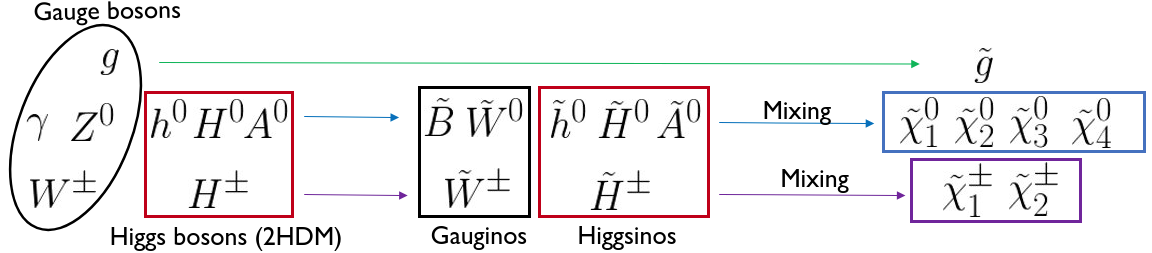
\includegraphics[width=\linewidth]{SUSY.png}
    \caption{Diagram depicting SM force carriers to their MSSM counterparts. The gluon is directly symmetric to the gluino, Higgs bosons and the W boson to the Higgsinos and the charged Winos, respectively. The photon and Z boson are technically part of the $B$ and the $W^3$, thus are symmetric to the Bino and neutral Wino, respectively. The neutral components of the gauginos and Higgsinos mix to give rise to the neutralinos, likewise for the charged components to the charginos.}
    \label{fig:SUSY}
\end{figure}

The new global symmetry \textit{R-parity} is required due to the the quantum numbers known as baryon ($B$) and lepton ($L$) numbers in the SM not considered as fundamental symmetries. This statement is supported by $B$- and $L$- violating processes that are strongly constrained by experiment. R-parity is a conserved quantum number given by Equation (\ref{eq:MPrec})
\begin{equation}
    P_R=(-1)^{3(B-L)+2s}
    \label{eq:MPrec}
\end{equation}
where $s$ is the spin of the particle. This symmetry conveniently separates SM particles and sparticles in a way that the SM particles have $P_R=+1$ (even R-parity), whereas the sparticles all have $P_R=-1$ (odd R-parity) \cite{martin1997supersymmetry}. In MSSM, the conservation of $R$-parity comes from SUSY events as a pair-produced event \cite{aitchison2007supersymmetry}. \\

%\footnote{The gauge invariance required in the SM ``accidentally" \cite{martin1997supersymmetry} guarantees the conservation of such quantum numbers in most interactions.}

%-------------------------------------------------------------------------%
\chapter{The top squark and its production}
\label{chap:3}
%\section{The stop ($ \Tilde{t} $) and its production}
%-------------------------------------------------------------------------%
\section{Possible decay channels of the top squarks} 
\label{sec:stopDecay}
Just like the SM particles and their decay dictated by known symmetries and conservation laws, the decay of stops is dictated by the parameters and kinematics suggested by MSSM. The mass of stops would significantly affect the decay modes. \\

A heavy enough stop at the order of the sum of the top quark mass and neutralino mass ($m_t+m_{\Tilde{\chi}_1^0}$) would undergo a two-body decay into top quarks with neutralinos: $\Tilde{t}_1\rightarrow t\Tilde{\chi}_1^0$. In the case where the neutralino is instead the chargino, the decay results in bottom quarks with charginos: $\Tilde{t}_1\rightarrow b\Tilde{\chi}_1^+$) \cite{boehm2000decays}. A lighter stop that is above the sum of the bottom quark mass, W-boson mass and neutralino mass ($m_b + m_W + m_{\Tilde{\chi}_1^0}$) would imply a three-body decay $\Tilde{t}_1\rightarrow b W \Tilde{\chi}_1^0$. Four-body decays into a combination of bottom quarks, neutralinos and SM fermions, may also be possible: $\Tilde{t}_1\rightarrow b\Tilde{\chi}_1^0 f \Bar{f}'$ \cite{boehm2000decays}. However, the four-body decay is only relevant when the two- and three-body decays are kinematically forbidden. This would also allow a flavor-suppressed decay to a charm quark: $\Tilde{t}_1\rightarrow c\Tilde{\chi}_1^0$ \cite{aad2014search}. \\

An important assumption made in these decays is that the stops are heavier than the neutralino mass ($m_{\Tilde{t}_1} > m_{\Tilde{\chi}_1^0} $) so that the neutralinos remain the lightest (LSP). Additional decays become apparent when sparticles other than $\Tilde{\chi}_1^0 $ are lighter than the stop, for example, the charginos $\Tilde{\chi}_1^{\pm}$. A diagram from \cite{aad2014search} is shown in Figure \ref{fig:decayMode}, that represent the statements above under the assumption that $ \Tilde{\chi}_1^0 $ and $\Tilde{t}_1 $ are the lightest and next-lightest particles in the MSSM. For the purpose of this project, we stick to a simplified model where the right-handed\footnote{The SM quarks have a left- and right-handed component in which they are a doublet and a singlet respectively. The MSSM counterpart follows this convention and the mixing of the two states provide two distinct squarks. The doublet allows mixing with other quarks (e.g. tops with the bottom) thus making them more complicated and potentially heavier.} stops mix to form the lighter stop. Furthermore, the decays we explore also follows the simplified model, where our desired background events is the process given by Equation (\ref{eq:background}) and the desired signal events given by Equation (\ref{eq:signal}). The final state includes one charged lepton, some missing energy and some hadronic jets, one which that originates from the $b$-quark at a minimum, as shown in Figure \ref{fig:stopDecay}.\\


\begin{figure}[htbp]
    \centering
    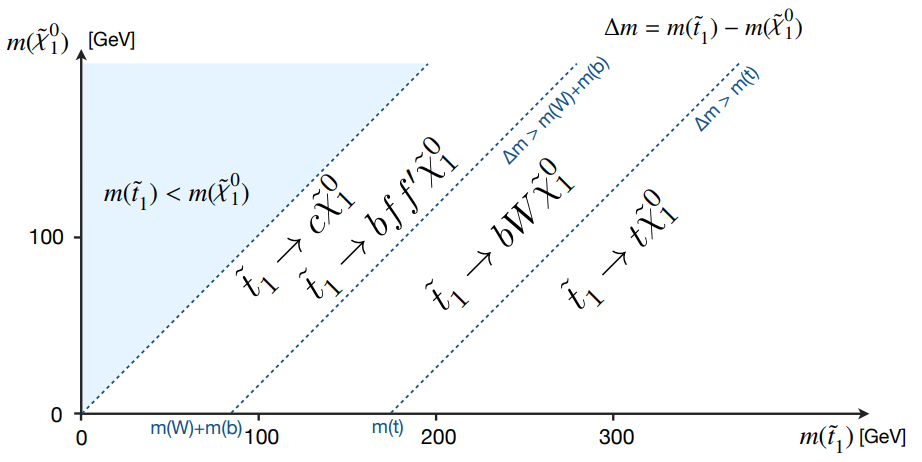
\includegraphics[width=0.75\linewidth]{decaymodes.png}
    \caption{Possible decay modes for stops within the mass-parameter space of $\Tilde{t}_1 $ and $ \Tilde{\chi}_1^0 $ \cite{aad2014search}. The blue filled region is kinematically forbidden due to the neutralino mass being heavier than the stop mass thus resulting in stops that are not energetic enough. As the mass of stops get heavier, the allowed decays differ due to its varying allowed kinematics, favoring on-shell decays over off-shell decays.}
    \label{fig:decayMode}
\end{figure}

\begin{equation}
 pp \rightarrow t \Bar{t} \rightarrow b\Bar{b}jjl\cancel{\it{E}}_{T},
 \label{eq:background}
\end{equation}
\begin{equation}
  pp \rightarrow \Tilde{t}\Tilde{t^*} \rightarrow t \Bar{t} \Tilde{\chi^0_1}\Tilde{\chi^0_1} \rightarrow b\Bar{b}jjl\cancel{\it{E}}_{T},
  \label{eq:signal}
\end{equation}

\begin{figure}[htbp]
    \centering
    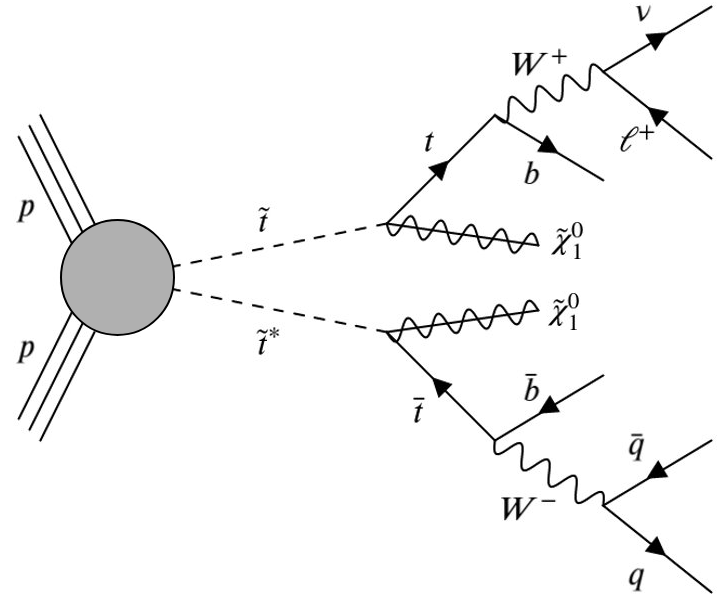
\includegraphics[width=0.5\linewidth]{stop_decay2.png}
    \caption{Decay chain of the signal of interest $\Tilde{t}\Tilde{t}^* \rightarrow t\bar{t}\Tilde{\chi}_1^0\Tilde{\chi}_1^0 $ with a final of state of one charged lepton and hadronic jets originating from the quark-antiquark pair and bottom quarks.}
    \label{fig:stopDecay}
\end{figure}
%-------------------------------------------------------------------------%
%\section{Mass of the top squark}
%\label{sec:stopMass}
%The mass eigenstates for the top squarks are given by the equation

%\begin{align}
%    \begin{pmatrix} \Tilde{t}_1 \\ \Tilde{t}_2 \end{pmatrix} = 
%    \begin{pmatrix} \cos\theta_\Tilde{t} & -\sin\theta^*_\Tilde{t} \\ \sin\theta_\Tilde{t} & \cos\theta^*__\Tilde{t} \end{pmatrix}
%    \begin{pmatrix} \Tilde{t}_L \\ \Tilde{t}_R \end{pmatrix}
%    \label{eq:stopMass}
%\end{align}
%where $ \theta_\Tilde{t} $ is the stop mixing angle in the range $ 0 \leq {\theta_\Tilde{t}} \leq \pi $ satisfying $ |\cos\theta_{\Tilde{t}}|^2 + |\sin\theta_{\Tilde{t}}|^2 = 1 $ \cite{martin1997supersymmetry}. \\

%The mass splitting of the two stops $ \tilde{t}_1 $ and $ \tilde{t}_2 $ arise from the squared-mass matrix for stops, where the off-diagonal elements involves a large top-quark Yukawa coupling ($y_t$ term) that induces such a phenomena \cite{kraml2016scalar}. Diagonalizing gives the $\Tilde{t}_L$ and $\Tilde{t}_R$ components on the right-hand side of Equation (\ref{eq:stopMass}). One possible model in the MSSM predicts that $\Tilde{t}_1$ is the lightest of all squarks, predominantly theorized to be $\Tilde{t}_R$ which is the right-handed stops \cite{martin1997supersymmetry}. Although there has been no success in the direct detection of the particle, experimental efforts have been made to set constraints on its mass \cite{kraml2016scalar, aad2014search, abdughani2018probing, sirunyan2018search, yoshihara2017search}.

%-------------------------------------------------------------------------%
\section{Mass parameters for the top squarks and neutralinos}
Experiments at the Large Hadron Collider have set limits on the stop mass and neutralino mass since operation begun in 2008. Many searches involving other exotic particles and its properties have been performed, thus how do particle physicists create such limits, and in the lucky scenario such as the Higgs boson, claim a discovery? In short, a frequentist approach\footnote{A Bayesian approach can also be taken, where it makes use of the posterior probability known as Bayes' theorem. It is said to have a wider range of applicability due to its ability to account for unknown parameters which frequntist approaches cannot, and differs greatly in its interpretation when claiming a discovery \cite{lista2017statistical}.} can be taken where the statistical analysis relies on likelihood-based hypothesis testing.

%-------------------------------------------------------------------------%
\subsection{Frequentist statistics - setting limits in searches}
\label{sec:freqStat}
A likelihood function provides us with the probability distribution function evaluated for the observed data, in which the extended likelihood function to account for the Poisson distribution of the number of events $N$ is given by
\begin{equation}
    L(\vec{x}_1,...,\vec{x}_n; \vec{\theta}) 
    = \frac{e^{-\mu_n(\vec{\theta})}\mu_n(\vec{\theta})}{n!}\prod^n_{i=1} f(\vec{x}_i;\vec{\theta})
    \label{eq:genLikelihood}
\end{equation}
where $\vec{x}_i$ is an individual observation in a set of $i=1,...,n$ random variables amongst $N$ number of uncorrelated events, $\mu_n(\vec{\theta})$ is the expected number of events dependant on some nuisance parameter $\vec{\theta}$, a parameter in which unknown parameters coupled to the parameter of interest from detector response is accounted for \cite{lista2017statistical}. When a background-only hypothesis $H_0$ is given as $\mu_n(\vec{\theta})=b$, then the alternate hypothesis  $H_1$ includes both signal and background events such that $\mu_n(\vec{\theta})=\mu s+b$. The likelihood function (\ref{eq:genLikelihood}) is then a parameter of $\mu$ i.e. $L(\mu,\vec{\theta})$, with $\mu=0$ corresponding to $H_0$ and $\mu=1$ to $H_1$. \\

We can obtain the profile likelihood ratio for the evaluated hypotheses with $H_0 \rightarrow L_{s+b}$ and $H_1 \rightarrow L_b$ into
\begin{equation}
    \lambda(\mu) = \frac{L_{s+b}(\mu, \hat{\hat{\theta}})}{L_b(\hat{\mu},\hat{\theta})}
    \label{eq:genLR}
\end{equation}
for some maximum-likelihood estimators\footnote{The maximum likelihood estimators provide the parameter values that maximize the search for a particular observation within the set.} $\hat{\mu}$ and $\hat{\theta}$, and $\hat{\hat{\theta}}$ being the conditional maximum-likelihood estimator \cite{cowan2011asymptotic}. The value for $\lambda$ rests between the range $0 \leq \lambda \leq 1$ which can be applied for some test statistic $q_\mu$\footnote{The signal discovery test statistic is $q_0$ where it holds the value $-2 \ln \lambda (0)$ for $\hat{\mu}=0$ and zero otherwise.} defined as
\begin{equation}
    q_\mu = \left\{
        \begin{array}{ll}
            -2\ln \lambda(\mu) & \quad \hat{\mu} \leq \mu \\
            0 & \quad \hat{\mu} \geq \mu
        \end{array}
    \right.
\end{equation}
where the larger the value $q_\mu$ is, the more likely the hypothesis whose value is represented by $\mu$ is incompatible with the data. This allows us to compute the significance\footnote{For a discovery to be claimed, particle physicists require a minimum of $Z=5$ that corresponds to $p=2.87\times10^{-7}$ when rejecting the background only hypothesis.} $Z$ and its associated $p$-value with the relationship
\begin{equation}
    Z = \Phi^{-1}(1-p) = \sqrt{q_\mu}
    \label{eq:Z}
\end{equation}
The exclusion of the hypothesis $\mu$ is supported when a threshold $p=\alpha$ is applied with a low value e.g. $\alpha=0.05$ for a 95\% confidence level ($Z=1.64$) \cite{cowan2011asymptotic}. \\

Collider experiments are considered a form of counting experiments, thus the observed events are categorized under a Poisson distribution with a mean of $\mu_s+\mu_b$ where $\mu_{s(b)}$ is the estimated number of signal(background) \cite{lista2017statistical, adam-bourdarios_learning_2014}. This gives us a more simplified version to Equation (\ref{eq:genLikelihood});
\begin{equation}
    P(n|\mu_s,\mu_b) = \frac{(\mu_s+\mu_b)^n}{n!}e^{-(\mu_s+\mu_b)}
    \label{eq:Poisson}
\end{equation}
whose likelihood ratio is given by
\begin{equation}
    \lambda = \frac{P(n|\mu_s,\mu_b)}{P(n|\hat{\mu_s},\mu_b)}
    \label{eq:likelihoodRatio}
\end{equation}
where $\hat{\mu_s}$ is the maximum likelihood estimator of $\mu_s$. \\


%-------------------------------------------------------------------------%
\subsection{Exclusion limits for the stop and neutralino masses}
The exclusion of masses for new exotic particles are performed according to rigorous statistic that Section \ref{sec:freqStat} has only touched a small portion of. The exclusion of stop and neutralino masses is visually presented as an exclusion curve in CMS and ATLAS, such as those seen in Figure \ref{fig:limits} \cite{cms2019search} where \textit{inside} the expected limit (in red) and observed limit (in black) have already been searched for and excluded. \\

\begin{figure}[htbp]
    \centering
    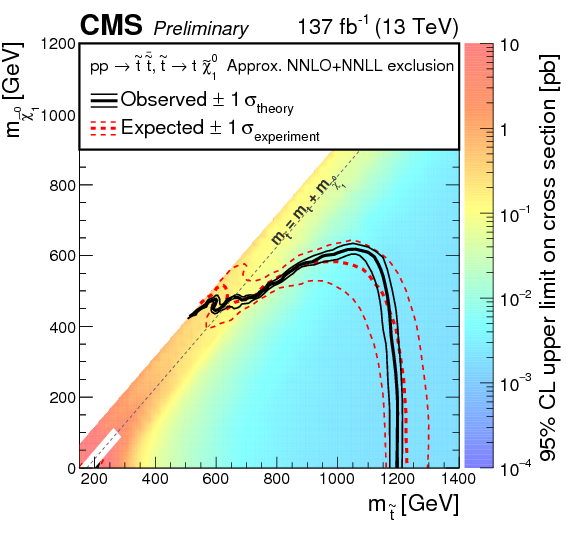
\includegraphics[width=12cm, height= 12cm]{stop_limits.png}
    \caption{The latest cross-section and mass limits for the process $\Tilde{t}\Tilde{t}^* \rightarrow t\bar{t}\Tilde{\chi}_1^0\Tilde{\chi}_1^0 $ set by the CMS experiment \cite{cms2019search}. Inside the black curve is the observed excluded masses for stops and neutralino, and outside this line remains a plausible region for masses for these particles, with the stop mass' limit pushed to the TeV scale. According to the color bar, the further out into to parameter space we travel to, the allowed cross-section is allowed.}
    \label{fig:limits}
\end{figure}

In this particular figure, it is presented that the expected limit to the process $pp \rightarrow \tilde{t}\tilde{t}^* \rightarrow t\tilde{\chi}_1^0$ falls under that of the observed limit when both masses are high i.e.  when stop masses are in the order of $1\sim1.2$TeV and neutralino masses in the order of $\sim600$ GeV. It is also shown that the observed limit falls under the expected limit when the mass there is a massive mass difference between the stop and the neutralino i.e. $m_{\tilde{\chi}_1^0}\ll m_{\tilde{t}}$. These two points indicated that a large mass difference between the two particles can is preferred at the current limits. Furthermore, the upper limit on the cross-section for the production of this process is provided in color-code, such that the values that fall above cross-sections and its corresponding colour will be excluded. This implies that our signal selection efficiency is high when searching in regions with weaker limit. \\

The path sitting around $ m_{\tilde{t}} \approx 1.2$ TeV is an interesting path to follow, and observe how the algorithms (in which this will be discussed in detail in a later section) perform. In addition, reference \cite{roxlo2018opening} have explored the performance of their neural networks discriminating stop production to top production, albeit in a dilepton final state within the $\tilde{t} \rightarrow t \tilde{\chi}_1^0$ decay. Their choice of mass parameters are set as the parameters our fourth benchmark explores: $m_{\tilde{t}} =750$ GeV and $m_{\tilde{\chi}_1^0} = 1$ GeV, well within the exclusion limit in Figure \ref{fig:limits}. Table \ref{tab:benchmarks} shows a summary of mass parameters chosen to explore. In particular it would be interesting to observe the behavior of the classifiers when the deviation for stop masses is slight opposed to a large deviation in neutralino masses. Intuitively, the large difference would imply that the final states will carry a large excess of missing energy, thus allowing the algorithm to distinguish them easily and allowing us to observe the physical behavior. 

\begin{table}[htbp]
    \centering
    \begin{tabular}{c|c|c|c} 
    \toprule
    Benchmark No. & Position & $\Tilde{t}$ Mass (TeV) & $\Tilde{\chi}_1^0$ Mass (GeV) \\
    \midrule
    \rowcolor{gray!6} 1 & Outside & $ 1.2 $ & $ 600 $ \\
    2 & Outside & $ 1.225 $ & $ 400 $ \\
    \rowcolor{gray!6} 3 & Outside & $ 1.25 $ & $ 100 $ \\
    4 & Inside & $ 0.75 $ & $ 1 $\\
    \bottomrule
    \end{tabular}
    \caption{Chosen parameters for building classifiers, three of which tracing just outside of the observed exclusion limit in Figure \ref{fig:limits}, and one of which is completely inside the curve, following that of \cite{roxlo2018opening}. In doing so we observe how the mass difference between the stops and neutralinos affect the production and sensitivity.} 
    \label{tab:benchmarks}
\end{table}



%-------------------------------------------------------------------------%
\chapter{Methods to search for MSSM}
\label{chap:4}
%\section{Methods to search for MSSM}
Research in high energy physics typically requires hadron colliders such as the Tevatron and the LHC as they can produce extremely high energies through proton-proton collisions. These collisions produce heavy particles with extremely short lifespans such as the top quark and W-bosons, making an ideal environment to study properties of heavy particles. This includes searches beyond the SM with SUSY and its sparticles. Located on the border of France and Switzerland, the LHC is the current world-leading facility for high energy physics collider experiments. The primary experimental collaboration for SUSY phenomena is the ATLAS (A Toroidal LHC ApparatuS) \cite{collaboration2008atlas} and CMS (Compact Muon Solenoid) \cite{chatrchyan2008cms} collaborations, where both collaborations at the LHC work independently of each other.

%-------------------------------------------------------------------------%
\section{The Large Hadron Collider and CMS}
The LHC currently operates at $ \sqrt{s}=13 \text{TeV} $, where the energy is $5-6$TeV higher than when the Higgs Boson was discovered. ATLAS and CMS are the general multi-purpose detectors at the LHC that conduct independent searches of high energy physics. Each detector is built slightly differently, allowing for variability in detection (although not too varying) to support any discoveries made at the LHC. \\

The CMS detector \cite{chatrchyan2008cms} weighs $12.5\times10^6$kg with a solenoid of 4T AND WRITE ABOUT PARAMETERS HERE. CMS has focused on a single large superconducting magnet. These detection parameters will be useful when considering kinematic variables associated importantly to stop production, just as it was for SM particle productions.

%-------------------------------------------------------------------------%
\section{Simulations of a collider}
Data collected in colliders do not initially contain a label regarding which physical process the entry corresponds to. A method to overcome this may be to individually observe each event and provide a corresponding label provided the correct understanding of the physics behind such processes. However, this is evidently inefficient and unrealistic. By performing simulations identical to the properties of the particle collider and closely following the production process with known theory and calculations, one may identify the process in the raw data using techniques such as ML. One program of such is MadGraph5 (MG5) \cite{alwall2014automated, alwall2011madgraph}, where the next-to-leading order differential cross-sections of an input event are generated at tree-level with Monte Carlo simulations. \\

The processes generated by MadGraph are known to be ``generator level", meaning the processes are only produced to what we specify it as, disregarding any physics that follow. Consequently, the events do not mimic an output of the detector exactly. In order to achieve a high resolution of detector simulations, these events must be processed further into what a real detector may observe. \\

%\section{Parton Showers with Pythia and detector simulation with Delphes}
A program called PYTHIA8.2 \cite{sjostrand2015introduction}has the functionality to extend the decays produced by MadGraph in a physical process known as parton showers. Intended to describe all components - such as elastic, diffractive, and non-diffractive topologies - of the total cross-section in collisions for soft processes, PYTHIA also includes capabilities such as \textit{parton distributions}, \textit{parton showers}, \textit{multi-parton interactions} and its own \textit{hard processes} such as QCD, electroweak and SUSY processes. Multi-parton interactions are not necessarily relevant to maintain in our processes, so by turning this feature off we save computation time. \\
%The user manual and website for the latest release (PYTHIA8.2) is recommended for readers who are interested in the specifics \cite{sjostrand2015introduction}, although more comprehensive physics are stated in the older version PYTHIA6.4. 

Delphes is the detector level simulation chosen for this project, due to its MadGraph build-in making the generation process smooth. The package allows us to choose either the ATLAS or CMS detector to simulate, in which CMS was chosen due to our parameters following those of CMS papers.


%-------------------------------------------------------------------------%
\section{Kinematic variables in collider experiments}
Data at the LHC is collected by taking measurements of the properties of particles resultant particles in the transverse plane to the beam direction. Considering the beam direction to be the z-direction the transverse plane would be the $(x,y)$-plane, with the geometry of this depicted in Figure \ref{fig:beam}. \\

\begin{figure}[htbp]
    \centering
    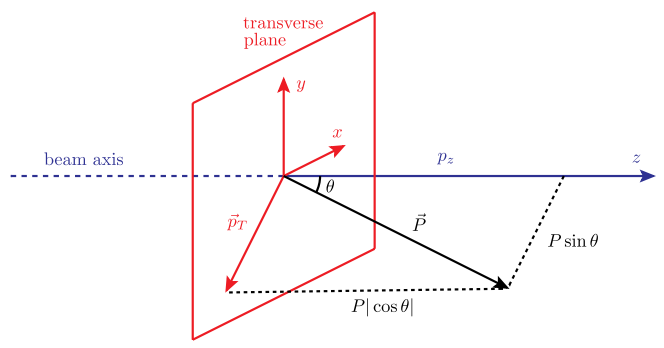
\includegraphics[width=12cm, height= 6cm]{beam.png}
    \caption{The geometry of a collider experiment, with the beam axis considered as the z-direction and the transverse plane as the $(x,y)$-plane \cite{barr2011guide}.}
    \label{fig:beam}
\end{figure}


A well summarized guide to the transverse plane and variables considered is given in reference \cite{barr2011guide}, where there are three types of projection methods - \textit{Mass-preserving}, \textit{Speed-preserving} and \textit{Massless}. The principal component being the transverse momentum given by Equation (\ref{eq:pt})
\begin{equation}
    p_T = \sqrt{p_x^2 + p_y^2}
    \label{eq:pt}
\end{equation}
maintains equivalence across the three types, the mass projections defer between the three. \\

An important variable to discriminate background and signals in collider experiments is the \textit{missing transverse energy} denoted as $\cancel{\it{E}}_{T}$, where it is, in general, the negative of the vector sum of the $p_T$ components reconstructed in the detector \cite{cms2011missing}. In the SM decays, leptonic decays produce their neutrino counterparts that freely passes through the detector, resulting in some $\cancel{\it{E}}_{T}$. Many SUSY events are predicted to have a large excess of $\cancel{\it{E}}_{T}$ moreso than the SM processes, due to a larger excess of undetectable particles. The reconstruction of the $\cancel{\it{E}}_{T}$ is sensitive to slight deviations such as mismeasurements and cosmic-ray particles.  %One may also consider the \textit{stransverse mass} denoted as $M_{T2}$ when searching for particles beyond SM. This observable places a maximal lower bound on the almost-invisible parent particles that decayed into detected particles \cite{lester2011stransverse}. These are only a few of many variables that could be used for analyses and will require further reading and careful exploration for potential candidates for the project.



%-------------------------------------------------------------------------%
\section{Possible search regions for the top squarks}


\begin{equation}
 pp \rightarrow t \Bar{t} \rightarrow b\Bar{b}jjl\cancel{\it{E}}_{T},
 \label{eq:background}
\end{equation}
\begin{equation}
  pp \rightarrow \Tilde{t}\Tilde{t^*} \rightarrow t \Bar{t} \Tilde{\chi^0_1}\Tilde{\chi^0_1} \rightarrow b\Bar{b}jjl\cancel{\it{E}}_{T},
  \label{eq:signal}
\end{equation}


The possible decay modes were discussed in Section \ref{sec:stopDecay}, but we were yet to fully encounter the possible decays that could correspond to the background. A well-summarized discussion about the possible backgrounds in stop production is presented in \cite{plehn2010stop}, where there are four possible modes suggested: top-pair, QCD, W+jets, and Z+jets. Note that \textit{jets} are some cluster of hadronized quarks or gluons produced in a decay since they cannot exist freely. They are used for analysis since they are well-defined, easily-to-measure/calculate and have a close correspondence to the final state of interest \cite{seymour1996jets}. \\

Quoted as ``dangerous", the top-pair production, especially the semi-leptonic top decays that we consider in this section, overwhelm the stop signals even after top-tagging (jets identified to have originated from top-decays) and signal selections made \cite{plehn2010stop}. The QCD background is said to be an``insurmountable" background at the LHC. However, it can be suppressed until below that of the $t\Bar{t}$ background by applying treatments such as ``fake" missing energy and $b$-mistagging (jets misclassified to have originated from b-quarks) and two top-tagging \cite{plehn2010stop}. The W+jets case is easier to deal with due to the apparent missing energies created from the four hard jets (plus others) that only marginally exceed that of the signal \cite{plehn2010stop}. These are dealt with basic cuts and two top-tagging \cite{plehn2010stop}. Finally, the Z+jets case can be deemed as irrelevant simply due to its significantly smaller rate \cite{plehn2010stop}. Of course, background derived from other processes will be produced in LHC experiments, however, the signatures will be different from how it originates, thus allowing the search to be narrowed down to identical processes in background and signal. From these, it is evident that the most interesting and pressing background decay to study is the semi-leptonic final state of the top quark decay. \\

The process of collider simulations includes generating the desired background and signals through the appropriate decay channels which can then be distinguished later on through machine learning techniques. For the purpose of this project, our desired background event would be the process $ pp \rightarrow t \Bar{t}$ and the desired signal event would be the process $ pp \rightarrow \Tilde{t}\Tilde{t^*} $. This section will expand on these event generations using MadGraph5, where I have run the program to produce the plots as a preliminary. \\

\begin{figure}[htbp]
    \centering
    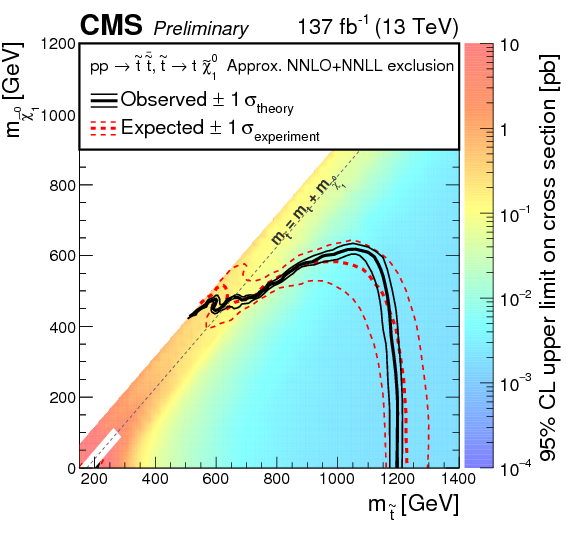
\includegraphics[width=12cm, height= 13cm]{stop_limits.png}
    \caption{The latest cross-section limit for the top squark presented in 
    \cite{cms2019search}}
    \label{fig:limits}
\end{figure}


\begin{table}
    \centering
    \begin{tabular}{c|c|c|c} 
    \toprule
    Benchmark No. & Position & $\Tilde{t}$ Mass (TeV) & $\Tilde{\chi}_1^0$ Mass (GeV) \\
    \midrule
    \rowcolor{gray!6} 1 & Outside & $ 1.2 $ & $ 600 $ \\
    2 & Outside & $ 1.225 $ & $ 400 $ \\
    \rowcolor{gray!6} 3 & Outside & $ 1.25 $ & $ 100 $ \\
    4 & Inside & $ 0.75 $ & $ 1 $\\
    \bottomrule
    \end{tabular}
    \caption{Chosen parameters for building classifiers} 
    \label{tab:benchmarks}
\end{table}

%-------------------------------------------------------------------------%
\chapter{Event generation - from pp collision to detection}
\label{chap:5}
%\section{Event generation - from the collision to detection}
%In this section, the method chosen to perform simulations for both the top and stop decays are shown. In addition, the preparation of data is explained to justify the usage of ML and their results.\\
%-------------------------------------------------------------------------%
\section{Background and Signal of interest}
\label{sec:production}
As discussed in Section \ref{sec:Sims}, MadGraph5 is the chosen software to perform particle collider simulations, in which one million events were produced for both the signal and background events. At the generator level, to meet the pre-selection criteria listed in the following subsection, we limit the missing transverse energy $\cancel{\it{E}}_{T}$ to a minimum of 200 GeV as the signatures significantly differ between our signal and backgrounds as seen in Figure \ref{fig:topMET}. From the histogram, it is evident that the background events have a distribution much closer to zero with a mean of roughly 50 GeV without this requirement. The difference in MET affects the results upon building the classifiers and efficiencies, thus by requiring the signatures to be in a similar range, we can observe the background events distributed closer to that of the signal, thus pushing the efficiency and sensitivity in our results to a reasonable range. In addition, MG5 calculates a cross-section value associated with each process generated, also required for our analysis. \\

\begin{figure}[htbp]
    \centering
    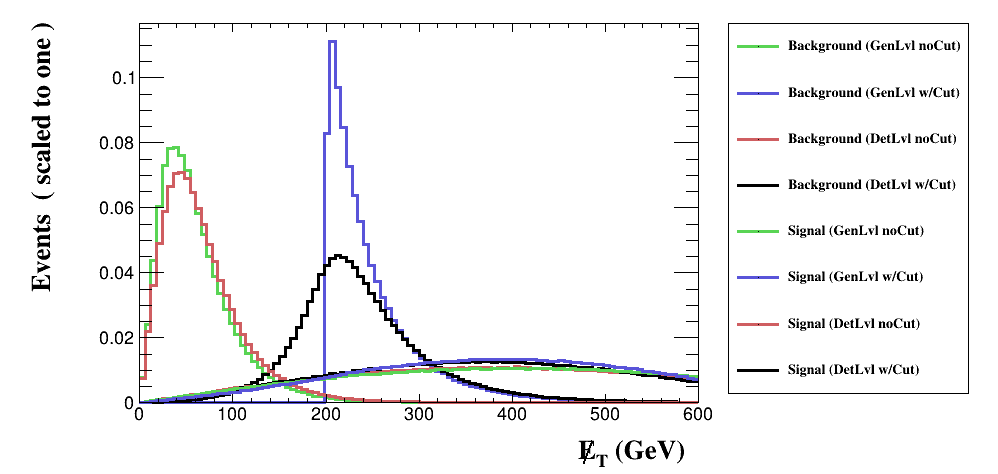
\includegraphics[width=\linewidth]{top-MET_new.png}
    \caption{A histogram to depict the variation in generator-level and detector-level simulation in the top quark production $pp \rightarrow t\Bar{t} \rightarrow bW^{-}\Bar{b}W^{+} \rightarrow l^{\pm}\nu_l(\Bar{\nu}_l)q\Bar{q}$, created using MadAnalysis5 \cite{conte2013madanalysis, conte2014designing, dumont2015toward}. In the legend, the terms `GenLvl noCut' refers to the events plotted with the LHE file corresponding to the hard process alone without placing the requirement $\cancel{\it{E}}_{T}>200$ GeV. Thus the lines represented with the term `w/Cut' corresponds to events simulated with this requirement. Furthermore, the detector effects on these events can be seen associated to those with `DetLvl'. By placing the requirement of $\cancel{\it{E}}_{T}>200$ GeV we observe the missing energy for our background shifts closer to the distribution for our signal events. Note that the signal used in this event is the first benchmark point with masses $m_{\Tilde{t}} = 1.2$ TeV and $m_{\Tilde{\chi}_1^0} = 600$ GeV.}
    \label{fig:topMET}
\end{figure}

Since the decay process involves both leptonic and hadronic particles as seen in Figure \ref{fig:topdecay}, the following were defined to make the simulation complete. \\

\begin{lstlisting}[mathescape = true]
        define leptonic = l+ l- ta+ ta- vl vl$\sim$
        define hadronic = u c d s u$\sim$ c$\sim$ d$\sim$ s$\sim$ b b$\sim$
\end{lstlisting}

For the background process defined by Equation (\ref{eq:background}), the command to generate the events is given by
\begin{lstlisting}[mathescape = true]
            generate p p > t t$\sim$ , 
            (t > W+ b , W+ > leptonic leptonic), 
            (t$\sim$ > W- b$\sim$, W- > hadronic hadronic)
        
            add process p p > t1 t1$\sim$ ,
            (t > W+ b , W+ > hadronic hadronic), 
            (t$\sim$ > W- b$\sim$, W- > leptonic leptonic)
\end{lstlisting}
where a diagram from one of its generated events can be seen in Figure \ref{fig:bkrdFeyn}. \\

Similarly, the process for signal\footnote{The parameter card was taken from \url{http://lpsc.in2p3.fr/projects-th/recasting/susy-vs-vlq/ttbarMET/} \cite{kraml2016scalar} under `SUSY-R', only adjusting the masses for stops and neutralinos in our runs.} production follows that of Equation (\ref{eq:signal}), in which the command for generating the events is given by
\begin{lstlisting}[mathescape = true]
        generate p p > t1 t1$\sim$ ,
        (t1 > t n1, (t > W+ b , W+ > leptonic leptonic)),
        (t1~ > t$\sim$ n1, (t$\sim$ > W- b$\sim$, W- > hadronic hadronic))
        
        add process p p > t1 t1$\sim$ , 
        (t1 > t n1, (t > W+ b , W+ > hadronic hadronic)), 
        (t1$\sim$ > t$\sim$ n1, (t$\sim$ > W- b$\sim$, W- > leptonic leptonic))
\end{lstlisting}
with an accompanying example diagram given in Figure \ref{fig:sigFeyn}. \\

\noindent\begin{minipage}{\textwidth}
\centering
  \begin{minipage}[htbp]{0.45\textwidth}
    \centering
    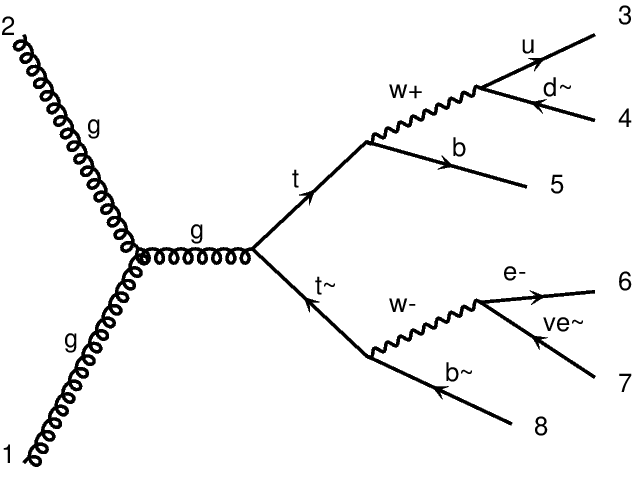
\includegraphics[width=\linewidth, keepaspectratio=true]{top_MG5.png}
    \captionof{figure}{Feynman diagram of the leading order background process $pp \rightarrow t \Bar{t} \rightarrow b\Bar{b}l^{+}jj\cancel{\it{E}}_{T} $.}
    \label{fig:bkrdFeyn}
  \end{minipage}
  \hfill
  \begin{minipage}[htbp]{0.45\textwidth}
    \centering
    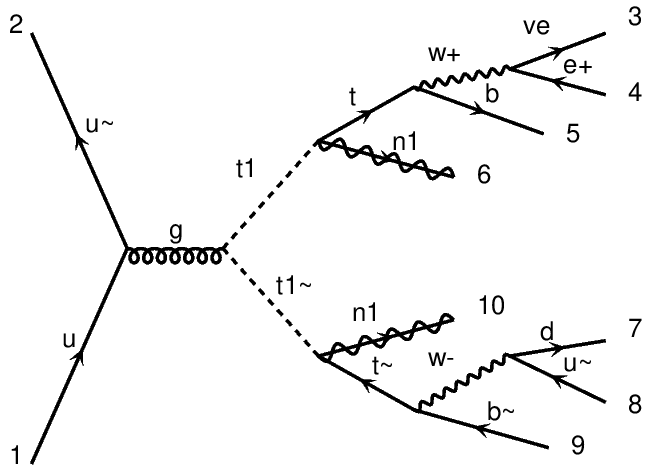
\includegraphics[width=\linewidth, keepaspectratio=true]{stop_MG5.png}
    \captionof{figure}{Feynman diagram of the leading order signal process $ pp \rightarrow \Tilde{t}\Tilde{t^*} \rightarrow t \Bar{t} \chi^0_1\chi^0_1 \rightarrow b\Bar{b}l^{+}jj\cancel{\it{E}}_{T} $ where the final states are identical to that of the background in Figure \ref{fig:bkrdFeyn}.}
    \label{fig:sigFeyn}
  \end{minipage}
\end{minipage}
%-------------------------------------------------------------------------%
\section{Preselection}
Applying existing conditions to searches reduces unwanted information, resulting in the algorithm working harder but allowing it to optimize its search for new physics. This process is known as \textit{pre-selection}, and it is a crucial step in our method. Rather, this process is identical to the cut-flow analysis seen in Section \ref{sec:cut}, where placing certain cuts allows us to reduce the number of events constrained to the signature of interest. During the pre-selection process we require three conditions the data must meet, based on several. 
\begin{itemize}
    \item $\cancel{\it{E}}_{T}>250$ GeV
    \item Only one charged lepton (No sign discrimination)
    \item A minimum of one $b$-tagged jet. The $b$-tagged jet with the highest $p_T$ is considered the only $b$-jet with the remainder considered as ordinary jets.\\
\end{itemize}

Table \ref{tab:benchmarks} depicts the number of events remaining after each pre-selection criteria applied, from left to right. The disparity in the initial events comes from the fact that we require an equal amount of data in the final count to have a 50:50 split between the signal and background events in our data. This allows our classifier to be built effectively. In addition, Table \ref{tab:benchmarks} lists the cross-section, $\sigma$, of each process simulated, which will be needed to evaluate important values that will be discussed in the following section. The cross-sections are shown to increase gradually as the mass difference between the stops and neutralinos becomes larger, showing that final states with more $\cancel{\it{E}}_{T}$ is less rare, although not by any substantial amount. \\

\begin{table}[htbp]
    \centering
    \begin{tabular}{c|c|c|c|c||c} 
    \toprule
    Data & Initial & $\cancel{\it{E}}_{T}>250$ GeV & $1l^\pm$ & $1b$ & Cross-section, $\sigma$ (pb) \\
    \midrule
    \rowcolor{gray!6} Benchmark1 & 776800 & 559371 & 179472 & 101488 & $1.6\times10^{-4} \pm 6.7\times10^{-8}$ \\
    Benchmark2 & 758458 & 611119 & 187179 & 101488 & $4.0\times10^{-4} \pm  5.4\times10^{-7}$ \\
    \rowcolor{gray!6} Benchmark3 & 758498 & 643458 & 191944 & 101488 & $6.6\times10^{-4} \pm 2.7\times10^{-7}$ \\
    Benchmark4 & 818636 & 515694 & 172171 &101488  & $4.0\times10^{-3} \pm 1.6\times10^{-6}$ \\
    \rowcolor{gray!6} Background & $10^6$ & 357273 & 123933 & 101488 & $2.5 \pm 1.3\times10^{-3}$ \\
    \bottomrule
    \end{tabular}
    \caption{The number of events remaining at each step of the pre-selection process. Requiring that events satisfy a minimum of 250 GeV for $\cancel{\it{E}}_{T}$, that there is only one charged lepton and one $b$-tagged jet, the number of events significantly differs between simulated signal and background events. Therefore the initial number of events was reduced for the signal events in order to create an equal split between signal and background within each data.} 
    \label{tab:preselection}
\end{table}



%-------------------------------------------------------------------------%
\chapter{Discriminating background and signal in the search regions}
\label{chap:6}
%\section{Discriminating background and signals with machine learning}
Machine learning (ML) is an increasingly popular data analytic technique widely employed in areas not limited to particle physics. It is useful for scenarios where a large amount of data generated or observed requires analyses that require better efficiency and computation time compared to traditional statistical techniques. In high energy physics, the use of machine learning has made a significant impact especially in the discovery of the Higgs boson using Boosted Decision Trees \cite{chatrchyan2012observation, aad2012observation, chen2015higgs}. However, machine learning is not an all-mighty tool that could discover new physics. \\


%-------------------------------------------------------------------------%
\section{Machine learning}
Machine learning is an umbrella term for algorithms that ``learns" patterns from a given data set whether small\footnote{There is a preferred limit to how small a dataset can be. For instance, for the number of entries $n$ and the number of variables $p$, if $n>p$ then there is not enough information for the classifier to train effectively.} or large to give predictions through a process called \text{training}. There are two general categories in ML, which are known as \textit{supervised learning} and \textit{unsupervised learning}. Supervised learning requires a separate data with labeled outcomes to build an effective model for analyzing the raw data whose outcomes are not labeled. Unsupervised techniques, on the other hand, are used when the data cannot have labeled outcomes making them purely data-driven methods, unlike supervised techniques. Supervised techniques are commonly employed in collider physics analysis as the simulation process allows as much data required to be generated, thus freely managing the size of data with labeled outcomes. This implies that balanced data can be created, as we have done in our method. \\

Training a dataset is relatively simple, with the choice of algorithm dictating how it is performed. Most existing open-source algorithms are user-friendly, extremely versatile and yield a high performance. Models are built by minimizing a chosen error, or a loss-function, where common choices are simple metrics such as the \textit{Mean Squared Error (MSE)}, 
\begin{equation}
    MSE = \frac{1}{n} \sum\limits_{i=1}^{n}(y_i-\hat{y}(x_i))^2
    \label{eq:MSE}
\end{equation}
or the \textit{Root MSE (RMSE)},
\begin{equation}
    RMSE = \sqrt{\frac{\sum\limits_{i=1}^{n}(y_i-\hat{y}(x_i))^2}{n}}
    \label{eq:RMSE}
\end{equation}
perform well in general. The error term is given by subtracting the predicted fit $\hat{y}_i$ at the $i$th observation to the ``true" fit $y_i$ \cite{james2013introduction}. Another high-performing loss-function is the negative log-likelihood function otherwise known as \textit{Log-Loss}
\begin{equation}
    l(x) = -\sum\limits_{i=1}^{n} \ln P(y_i| z_i) = \sum\limits_{i=1}^{n} \Big(-y_i z_i + \ln(1+e^{z_i}) \Big)
    \label{eq:logloss}
\end{equation}
for some regressor $z_i=\beta^T x_i$ for a given $i$th observation $x_i$.The log-loss function is derived from the logistic function $g(z_i)=1/(1+e^{-z_i})$, where $P(y_i| z_i) = g(z_i)^{y_i}(1-g(z_i))^{1-y_i}$ for a binary class problem with values $y_i=0,1$. This particular loss-function was chosen in this project after some preliminary runs through the datasets, yielding the best performance most consistantly. \\

When training a classifier one must be careful of \textit{overtraining}, a relatively common error that many encounters. Overtraining occurs when a model's parameters are too restrictive, limiting a model to be versatile in its performance. Versatility here relates to how a model performs under various datasets that are similar in nature. In other words, by restricting a model to perform well under a single dataset when training, we limit ourselves in performing well with predicting outcomes in cases such as the raw data. Overtraining is not a difficult mistake to avoid, and methods to improve the performance of a classifier conveniently assures this problem does not occur. Methods used in this project are known as \text{cross-validation} and \textit{hyperparameter grid-search}. \\

\begin{itemize}
    \item \textbf{Cross-Validation (CV)} \par
    Cross-validations (CV) is a task that requires the training data to be further partitioned to create a smaller set of training and test data. The most common CV technique is the \textit{k-fold CV}, where the training data is randomly sampled into $k$ different subsets. By selecting the $k-1$ of these subsets as the training data to build the classifier on, the remaining subset is used to validate this model. This procedure is repeated $k$ times through each split, where each performance is scored. The overall result typically involves taking the average of the $k$-fold scores.  There are no set rules on what the best value of $k$ is, however, most ML users prefer to stick to either 5 or 10 due to its simplicity and performance yield \cite{james2013introduction}. \\
    
    \item \textbf{Hyperparameter Grid-Search} \par
    Upon building a classifier, it is difficult to find the most optimal parameters whilst being cautious of overtraining. To overcome this dilemma, a grid search can be performed. A grid search utilizes CV at its foundations to test the performance of the selected parameters. By utilizing this feature, it is possible to check through a range of parameters. The down-side to this, however, is that it is computationally expensive and multiple evaluations may be required to even find some consistency in the results before narrowing down some parameters. \\
    
\end{itemize}


Fine-tuning parameters whilst cross-validating is not the only effective method to improve the classifier. A common technique known as \textit{feature engineering} can be employed to manipulate the existing variables so that the prediction accuracy may improve across the models built, although not guaranteed. In this work, a simple feature engineering was performed. This entailed of rearranging the four jet entries such that the highest $p_T$ jet with a b-tag is considered the b-jet originating from the decay, and the subsequent jets are ordered by the $p_T$ values regardless of whether there is a b-tag or not. \\

The most popular algorithms employed by the scientific community (not limited to physics) are Neural Networks (NNs) and Decision Trees (DTs). In the correct setting, either method performs exceptionally well. The trend in many communities favour NNs over DTs. However, through some preliminary tests using the \textit{h2o} package's \cite{h2o} \textit{automl} function, it was shown that a tree-based method known as \textit{Extreme Gradient Boosting (EGB/XGBoost)} is most suited for this task. The package that contains this feature is known as \textit{xgboost} , both available as a standalone use \cite{xgboost} or an extension of the h2o package \cite{h2o}. \\

%-------------------------------------------------------------------------%
\section{Tree-based methods and Extreme Gradient Boosting}
\label{sec:method}
Tree-based methods can intuitively be thought of as an extension to cut-flow analysis\footnote{See Section \ref{sec:cut}.}. Instead of discarding selections that do not fulfill certain criteria, these selections may be further explored upon by the algorithm provided that a new criterion exists. However, these splits are performed by minimizing a chosen loss-function as shown in the preceding section, thus making it difficult to infer the physical consequences of such splits. A simple diagram is depicted in Figure \ref{fig:tree}, where the mathematical form of a regression tree is described by
\begin{equation}
    f(x) = \sum_{i=1}^m c_i I(x\in R_i)
    \label{eq:DT}
\end{equation}
Here, $c_i$ is the coefficient associated to the partition of the data, $R_i$, for $m$ different partitions such that it is $c_i$ when $I(x\in R_i)$ is nonzero, and zero otherwise \cite{james2013introduction}. \\

\begin{figure}[htbp]
    \centering
    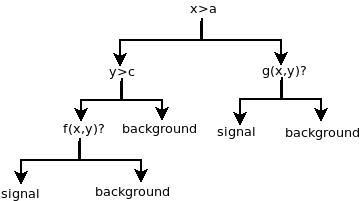
\includegraphics[width=10cm, height= 6cm]{DT.png}
    \caption{A simple decision tree for a hypothetical signal selection such that an extra parameter $g(x,y)$ is present within the algorithm. In Section \ref{sec:cut}, the partition criteria such as $x$ and $f(x,y)$ in cut-flow analysis were physically motivated and transparent. The algorithm makes this process somewhat of a black-box, making direct physical interpretations challenging.}
    \label{fig:tree}
\end{figure}

Many tree-based methods vary in the data sampling method and how a loss-function is minimized. In the case of EGB models, it is an extension to the \textit{Gradient Boosted Machine (GBM)} developed by Jerome Friedman \cite{friedman2001greedy}. \textit{Boosting} is an iterative algorithm in which an ensemble of weak models\footnote{A weak model consists of a small decision tree that is not an effective approximation to the data of interest.} are built sequentially, correcting its previous model through re-weighting. This leads to a final model that is highly representative of our data. Gradient boosting extends this idea such that a differentiable loss-function's gradient (known as gradient descent) allows the errors to reduce locally until the error is as close to zero as possible. EGB/XGBoost adds to the features of regular GBMs with weighted quantile splittings and its ability to manage sparse\footnote{Since there are no missing entries in this project, the data is not sparse, or rather, it is `dense'.} data, incorporating parallel computing to achieve faster computation time compared to regular GBM algorithms \cite{chen2016xgboost}. By also including regularization, a method to avoid overfitting by adding penalty terms to the loss-function, we were able to make its predictive power more reliable. \\
%-------------------------------------------------------------------------%
\section{Metrics for model performance}
\label{sec:metrics}
The performance of a classifier can be summarized into a single table known as a confusion matrix. Displayed in Table \ref{tab:ConfMat}, a confusion matrix visually shows the distribution of correctly and incorrectly classified points within the dataset. The correctly classified signal and background events are the True Positives (TP) and True Negatives (TN), respectively. Likewise, the incorrectly classified signal and background events are the False Negatives (FN) and False Positive (FP), respectively. The accuracy of the classifier is given by (TP+TN)/N and in a regression setting such as those in xgboost, a cut-off varies this value by a slight margin. Choosing the ideal cut-off is more important than achieving high accuracy, as we wish to maximize the Signal-to-Background Ratio (SBR)\footnote{The signal-to-background ratio is defined to be the proportion of signal over the proportion of background events. In our analysis, we look to the luminosity-normalized TP and FP rates for signal and background respectively.}\\

% Confusion matrix template
\begin{table}[htbp]
    \centering 
    \begin{tabu}{c|[2pt]c|c|c|c}
        \multicolumn{2}{c}{}&\multicolumn{2}{c}{Predicted}&\\
        \tabucline[2pt]{3-5}
        \multicolumn{2}{c|[2pt]}{}
        &\multicolumn{1}{c|}{Background} &\multicolumn{1}{c|[2pt]}{Signal} &\multicolumn{1}{c|[2pt]}{Total}\\
        \tabucline[2pt]{2-5}
        \multirow{\items}{*}{\rotatebox{90}{Simulated}}
        &\multicolumn{1}{c|[2pt]}{Background} & \multicolumn{1}{c|}{TN} & \multicolumn{1}{c|[2pt]}{FP} & \multicolumn{1}{c|[2pt]}{TN$+$FP} \\
        \cline{2-5}
        \multicolumn{1}{c|[2pt]}{}& \multicolumn{1}{c|[2pt]}{Signal} & \multicolumn{1}{c|}{FN} & \multicolumn{1}{c|[2pt]}{TP} & \multicolumn{1}{c|[2pt]}{FN$+$TP} \\
        \tabucline[2pt]{2-5}
        \multicolumn{1}{c|[2pt]}{} & \multicolumn{1}{c|[2pt]}{Total} & \multicolumn{1}{c|}{TN$+$FN} & \multicolumn{1}{c|[2pt]}{FP$+$TP} & \multicolumn{1}{c|[2pt]}{N}\\
        \tabucline[2pt]{2-5}
    \end{tabu}
    \caption{A confusion matrix for truth (simulated) and predicted labels and its components. The diagonal components are the correctly classified background (TN) and signal (TP) events. The off-diagonal components are the mis-classified background (FP) and signal (FN) events. }
    \label{tab:ConfMat}
\end{table}

An evaluation metric presented by the Higgs Challenge \cite{adam-bourdarios_learning_2014} is the \textit{approximate median significance (AMS)}, given by Equation \ref{eq:AMS}
\begin{equation}
    \text{AMS} = \sqrt{2\Big((s+b+b_r)\ln\Big(1+\frac{s}{b+b_r}\Big)-s\Big)}
    \label{eq:AMS}
\end{equation}
where $s$ and $b$ are the \textit{luminosity-normalized} TP and FP rates, respectively, and $b_r$ is a constant regularization term set at 10, found through preliminary results in the Higgs Challenge. Adding the regularization term places a bias toward larger selection regions, thus reducing the variance in the AMS value obtained. In order to obtain $s$ and $b$, we follow Equation (\ref{eq:N})
\begin{equation}
    s(b) = N_{s(b)}\times \epsilon_{s(b)} 
    \label{eq:N}
\end{equation}
where $N_{s(b)} = \sigma \int L(t) dt = \sigma \times 137$ \cite{thomson2013modern} is the number of expected events, and $\epsilon_{s(b)}=\text{TP(FP)}/\text{N}$ is the efficiency of the classifier given a dataset of size N, where in our case, would be a third of each dataset partitioned as our test set. The signal and background values when calculating the SBR we wish to maximize will refer to the value obtained via Equation (\ref{eq:N}) henceforth. \\

The Gaussian significance discovery, discussed briefly in Section \ref{sec:freqStat}, with an estimated standard deviation\footnote{The standard deviation is actually given by $(n-\mu_b)/\sqrt{\mu_b}$ as the Poisson fluctuation of the background has a standard deviation of $\sqrt{\mu_b}$. Here, $n$ is the number of events and $\mu_b$ is the mean of the background. These numbers are replaced with their empirical counterparts: $s+b$ and $b$ respectively.} of $s/\sqrt{b}$ only hold when $s \ll b$ and $b\gg1$. This is not true in practice, therefore we turn to an approximate measure such as the AMS. 
%This measure is a derivation of the significance Z given by Equation (\ref{eq:Z})
%\begin{equation}
%    \text{Z} = \sqrt{2\Big( n\ln\Big(\frac{n}{\mu_b}\Big)-n+\mu_b\Big)}
%    \label{eq:Z}
%\end{equation}
%where $n$ is the number of events and $\mu_b$ is the mean of the background, requiring that $n>\mu_b$. The values $n$ and $\mu_b$ are replaced by $s+b$ and $b$ in Equation (\ref{eq:AMS}), respectively. Traditionally, the Z significane at $Z=5$ corresponds to a $p$-value of less than $2.9\times10^{-7}$, sufficient to claim a discovery \cite{adam-bourdarios_learning_2014}. However, the regularization term $b_r$ is equal to zero in this setting, thus differing this significance of values given by either equations. \\
%-------------------------------------------------------------------------%
%\section{}


%-------------------------------------------------------------------------%

%-------------------------------------------------------------------------%
\chapter{Observing the physics of our models}
\label{chap:7}
%\section{Results}
%\begin{figure}[h!]
%    \centering
%    \includegraphics[width=14cm, height= 7.5cm]{.png}
%    \caption{}
%    \label{fig:}
%\end{figure}

%-------------------------------------------------------------------------%
\section{Performance of the classifiers}
%-------------------------------------------------------------------------%
%\subsection{Benchmark 1: \texorpdfstring{$\Tilde{t} = 1.2$}{ } TeV and \texorpdfstring{$\Tilde{\chi}_1^0 = 600$}{ } GeV}
An initial measure to visually understand how our classifiers have performed, a simple Receiver operating characteristic (ROC) curve can be constructed. A ROC curve shows the distribution of the predicted values given between 0 and 1, as a function of FP rate versus TP rate. This allows us to understand how much error we are willing to accept/reject for a given model, where we can produce histograms to observe where the optimum cut-off may be (see Figures \ref{fig:dist_bm1}-\ref{fig:dist_bm_in}. The ROC curve produced for all four benchmark data is presented in Figure \ref{fig:ROC} showing excellent performance across. As expected, however, the benchmark set corresponding to mass parameters within the exclusion curve (benchmark4: $\Tilde{t} = 750$ GeV and $\Tilde{\chi}_1^0 = 1$ GeV) performed the worst amongst the four due to the smaller mass difference between the stops and neutralinos. We also note that the datasets performed better as the mass difference became larger, which is also an expected behavior as the larger mass difference creates more energetic (anti)tops, consequently, more missing energy. This allowed the classifier to pick up such signatures easily, and we suspect that the missing energy's magnitude is the most influential variable the classifier has used when performing its splits. \\


\begin{figure}[htbp]
    \centering
    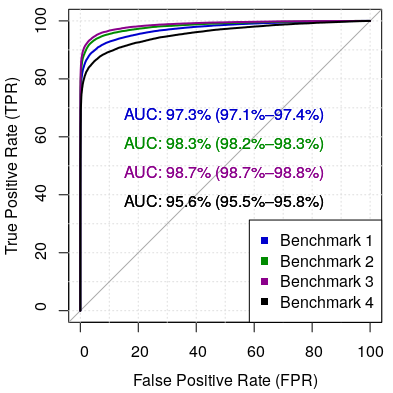
\includegraphics[width=0.4\linewidth]{ROC_curve.png}
    \caption{ROC curve for all 4 benchmark points. The forth benchmark corresponding to masses within the exclusion curve performed least well, where the remaining three performed slightly better when the mass difference between the stops and neutralinos became larger.}
    \label{fig:ROC}
\end{figure} 

Although the Area-under-the-curve (AUC) value is given in Figure \ref{fig:ROC}, it is maximized and does not directly represent the accuracy of our models. The accuracy of our models can be obtained by setting a cut-off to our predictions i.e. a number between 0 and 1. The closer the value is to 1 the lower the accuracy, but deliberately obtaining a high accuracy by setting a smaller value is also conter-intuitive as the Signal-to-Noise Ratio (SBR) will be smaller. Through various trials in cut-off values, it was determined for all four datasets that 0.75 is the optimal value to satisfy both high accuracy and high SBR. \\

For the benchmark point $\Tilde{t} = 1.2$ TeV and $\Tilde{\chi}_1^0 = 600$ GeV, the classifier performed quite well, producing a result of above $90\%$ accuracy. It is expected that the classifier performed less accurately when dealing with signal-like events. It correctly identified a smaller portion of true signal events and incorrectly classified more signal-like background events, as seen in Table \ref{tab:Values1}. The number of expected number of signal is significantly less than the expected number of background, producing an AMS value of 0.1. Considering the definition of AMS given in Section \ref{sec:metrics}, it supports the exclusion limit in Figure \ref{fig:limits}. \\

\noindent\begin{minipage}{\textwidth}
\centering
  \begin{minipage}[htbp]{0.6\textwidth}
    \centering
    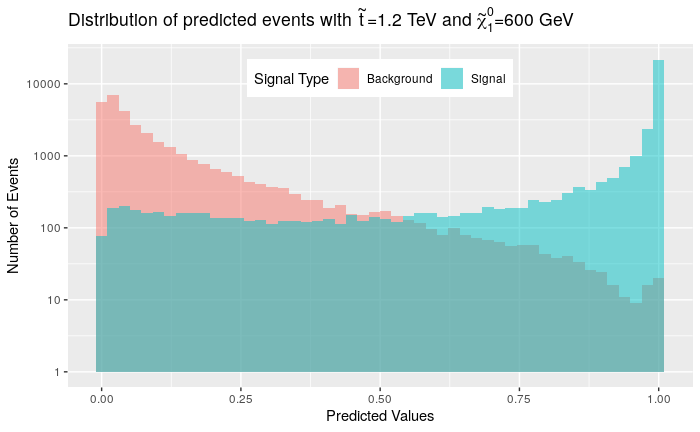
\includegraphics[width=\linewidth]{bm1_distribution.png}
    \captionof{figure}{Distribution of predicted background (pink) and signal (blue) events. The signal has a sharp drop-off at higher cut-off values unlike the background steadily, almost linearly, decreasing in number toward higher values. Note that y-axis is in a $\log_{10}$ scale.}
    \label{fig:dist_bm1}
  \end{minipage}
  \hfill
  \begin{minipage}[htbp]{0.39\textwidth}
        \centering
        \begin{tabular}{c|c} 
        \toprule
        Metric & Proportion \\
        \midrule
        \rowcolor{gray!6} TP & $42.0 \%$ \\
        TN & $49.4 \%$ \\
        \rowcolor{gray!6} FP & $0.6 \%$\\
        FN & $8.0 \%$ \\
        \rowcolor{gray!6} Accuracy & $91.4 \pm 0.2 \%$ \\
        \midrule
        $b$ & $388$ \\
        \rowcolor{gray!6} $s$ & $2$ \\
        SBR & $0.52\%$\\
        \rowcolor{gray!6} AMS & $0.1$ \\
        \bottomrule
        \end{tabular}
        \captionof{table}{Proportion of correctly and incorrectly classified points with the number of expected events calculated with Equation (\ref{eq:N}). The ratio, SBR, and AMS (Equation (\ref{eq:AMS})) were also calculated.} 
        \label{tab:Values1}
    \end{minipage}
\end{minipage}
\hfill \break
%-------------------------------------------------------------------------%
%\subsection{Benchmark 2: \texorpdfstring{$\Tilde{t} = 1.225$}{ } TeV and \texorpdfstring{$\Tilde{\chi}_1^0 = 400$}{ } GeV}

\noindent\begin{minipage}{\textwidth}
\centering
  \begin{minipage}[htbp]{0.6\textwidth}
    \centering
    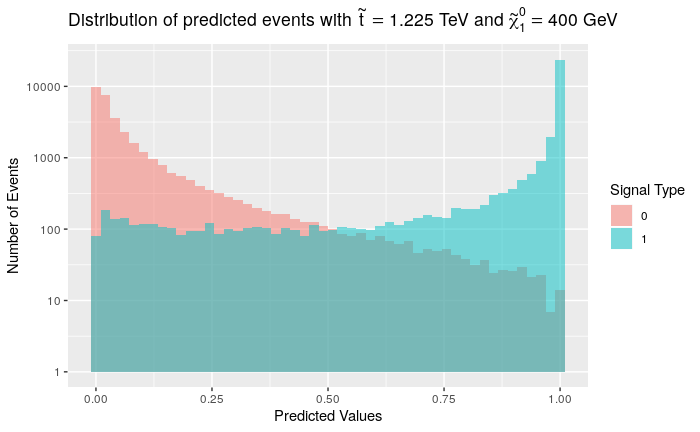
\includegraphics[width=\linewidth]{bm2_distribution.png}
    \captionof{figure}{Distribution of predicted background (pink) and signal (blue) events. The signal has a sharp drop-off at higher cut-off values unlike the background steadily, almost linearly, decreasing in number toward higher values. Note that y-axis is in a $\log_{10}$ scale.}
    \label{fig:dist_bm2}
  \end{minipage}
  \hfill
  \begin{minipage}[htbp]{0.39\textwidth}
        \centering
        \begin{tabular}{c|c} 
        \toprule
        Metric & Proportion \\
        \midrule
        \rowcolor{gray!6} TP & $43.8 \%$ \\
        TN & $49.5 \%$ \\
        \rowcolor{gray!6} FP & $0.5 \%$\\
        FN & $6.2 \%$ \\
        \rowcolor{gray!6} Accuracy & $93.3 \pm 0.2 \%$ \\
        \midrule
        $b$ & $362$ \\
        \rowcolor{gray!6} $s$ & $6$ \\
        SBR & $1.7\%$\\
        \rowcolor{gray!6} AMS & $0.31$ \\
        \bottomrule
        \end{tabular}
        \captionof{table}{Proportion of correctly and incorrectly classified points with the number of expected events calculated with Equation (\ref{eq:N}). The ratio, SBR, and AMS (Equation (\ref{eq:AMS})) were also calculated.} 
        \label{tab:Values2}
    \end{minipage}
\end{minipage}
\hfill \hfill \break
%-------------------------------------------------------------------------%
%\subsection{Benchmark 3: \texorpdfstring{$\Tilde{t} = 1.25$}{ } TeV and \texorpdfstring{$\Tilde{\chi}_1^0 = 100$}{ } GeV}

\noindent\begin{minipage}{\textwidth}
\centering
  \begin{minipage}[htbp]{0.6\textwidth}
    \centering
    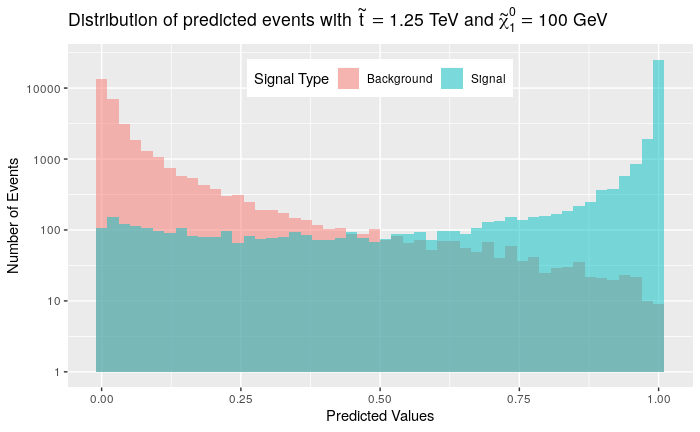
\includegraphics[width=\linewidth]{bm3_distribution.png}
    \captionof{figure}{Distribution of predicted background (pink) and signal (blue) events. The signal has a sharp drop-off at higher cut-off values unlike the background steadily, almost linearly, decreasing in number toward higher values. Note that y-axis is in a $\log_{10}$ scale.}
    \label{fig:dist_bm3}
  \end{minipage}
  \hfill
  \begin{minipage}[htbp]{0.39\textwidth}
        \centering
        \begin{tabular}{c|c} 
        \toprule
        Metric & Proportion \\
        \midrule
        \rowcolor{gray!6} TP & $44.9 \%$ \\
        TN & $49.5 \%$ \\
        \rowcolor{gray!6} FP & $0.5 \%$\\
        FN & $5.1 \%$ \\
        \rowcolor{gray!6} Accuracy & $94.4 \pm 0.2 \%$ \\
        \midrule
        $b$ & $323$ \\
        \rowcolor{gray!6} $s$ & $11$ \\
        SBR & $3.4\%$\\
        \rowcolor{gray!6} AMS & $0.6$ \\
        \bottomrule
        \end{tabular}
        \captionof{table}{Proportion of correctly and incorrectly classified points with the number of expected events calculated with Equation (\ref{eq:N}). The ratio, SBR, and AMS (Equation (\ref{eq:AMS})) were also calculated.} 
        \label{tab:Values3}
    \end{minipage}
\end{minipage}
\hfill\break
%-------------------------------------------------------------------------%
%\subsection{Benchmark 4: \texorpdfstring{$\Tilde{t} = 750$}{ } GeV and \texorpdfstring{$\Tilde{\chi}_1^0 = 1$}{ } GeV}

\noindent\begin{minipage}{\textwidth}
  \centering
  \begin{minipage}[htbp]{0.6\textwidth}
    \centering
    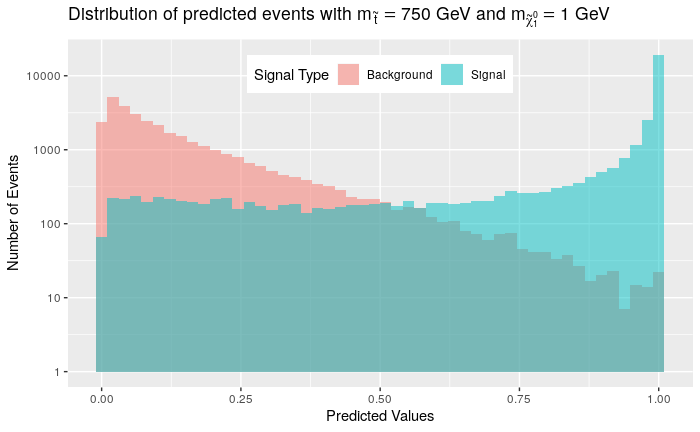
\includegraphics[width=\linewidth]{bm_In_distribution.png}
    \captionof{figure}{Distribution of predicted background (pink) and signal (blue) events. The signal has a sharp drop-off at higher cut-off values unlike the background steadily, almost linearly, decreasing in number toward higher values. Note that y-axis is in a $\log_{10}$ scale.}
    \label{fig:dist_bm_in}
  \end{minipage}
  \hfill
  \begin{minipage}[htbp]{0.39\textwidth}
        \centering
        \begin{tabular}{c|c} 
        \toprule
        Metric & Proportion \\
        \midrule
        \rowcolor{gray!6} TP & $39.4 \%$ \\
        TN & $49.6 \%$ \\
        \rowcolor{gray!6} FP & $0.4 \%$\\
        FN & $10.6 \%$ \\
        \rowcolor{gray!6} Accuracy & $89.0 \pm 0.2 \%$ \\
        \midrule
        $b$ & $343$ \\
        \rowcolor{gray!6} $s$ & $54$ \\
        SBR & $15.7\%$\\
        \rowcolor{gray!6} AMS & $2.8$ \\
        \bottomrule
        \end{tabular}
        \captionof{table}{Proportion of correctly and incorrectly classified points with the number of expected events calculated with Equation (\ref{eq:N}). The ratio, SBR, and AMS (Equation (\ref{eq:AMS})) were also calculated.} 
        \label{tab:Values_in}
    \end{minipage}
\end{minipage}
\hfill\break

\begin{table}[htbp]
    \centering
    \begin{tabular}{c||c|c}
        \toprule
        Metric & I.L. = $137\text{fb}^{-1}$ & I.L. = $35.9\text{fb}^{-1}$ \\
        \midrule
        \rowcolor{gray!6} $b$ & $343$ & $90$ \\
        $s$ & $54$ & $14$\\
        \rowcolor{gray!6} SBR & $15.7\%$ & $15.6\%$\\
        AMS & $2.8$ & $1.37$ \\
        \bottomrule
    \end{tabular}
    \caption{A table comparing values obtained with two different values for the integrated luminosity (I.L.), $137\text{fb}^{-1}$ and $35.9\text{fb}^{-1}$, within the mass parameter $\Tilde{t} = 750$ GeV and $\Tilde{\chi}_1^0 = 1$ GeV. Although the AMS values differ, the SBR is almost identical, showing that the sensitivity is no different across varying luminosity.}
    \label{tab:valsComp}
\end{table}
\hfill\break

The AMS value of 0.75 obtained by this benchmark is less than but close to the value found by Roxlo and Reece \cite{roxlo2018opening} which was 1.72. This is a reassuring result, as the exclusion limit shows that indeed this point is unlikely to be the mass parameters for both the stop and the neutralino. \\

XGBoost has an additional useful feature that calculates the \textit{feature importance} according to the \textit{Gain}, \textit{Cover} and \textit{Frequency} of each variable fed into building the classifiers \cite{xgboost}. We have used the metric `Gain' as it corresponds to the contribution of each variable based on the total gain they had when performing splits. We plot the variables accordingly, shown in Figure \ref{fig:imps} below. \\

\begin{figure}[htbp]
\centering
  \begin{minipage}[htbp]{0.45\textwidth}
    \centering
    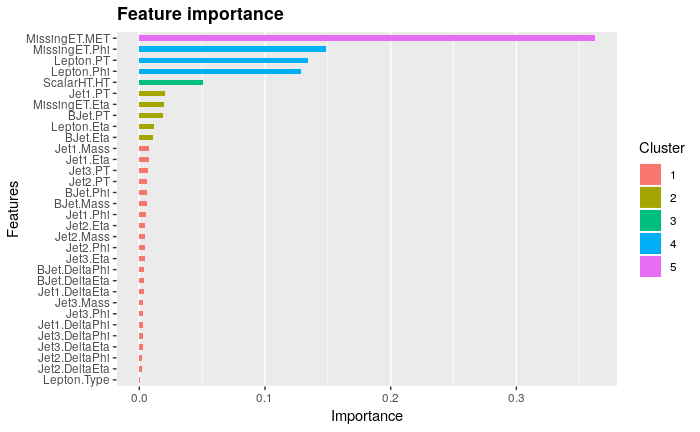
\includegraphics[width=\linewidth, keepaspectratio=true]{imp1.png}
    %\captionof{figure}{Feynman diagram of the leading order background process $pp \rightarrow t \Bar{t} \rightarrow b\Bar{b}l^{+}jj\cancel{\it{E}}_{T} $.}
    \label{fig:imp1}
  \end{minipage}
  \hfill
  \begin{minipage}[htbp]{0.45\textwidth}
    \centering
    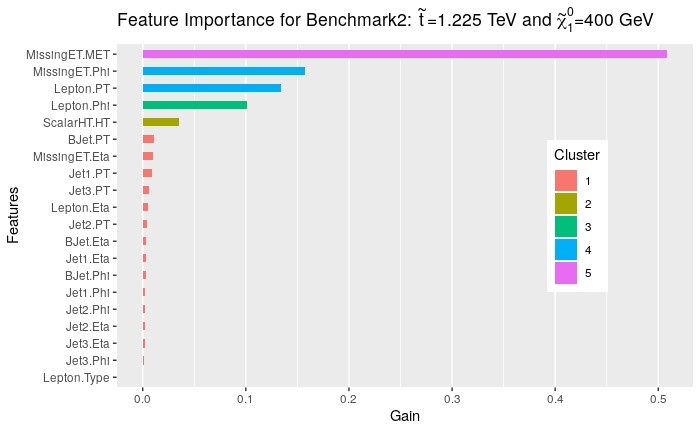
\includegraphics[width=\linewidth, keepaspectratio=true]{imp2.png}
    %\captionof{figure}{Feynman diagram of the leading order signal process $ pp \rightarrow \Tilde{t}\Tilde{t^*} \rightarrow t \Bar{t} \chi^0_1\chi^0_1 \rightarrow b\Bar{b}l^{+}jj\cancel{\it{E}}_{T} $ where the final states are identical to that of the background in Figure \ref{fig:bkrdFeyn}.}
    \label{fig:imp2}
  \end{minipage}
  \hfill
  \begin{minipage}[htbp]{0.45\textwidth}
    \centering
    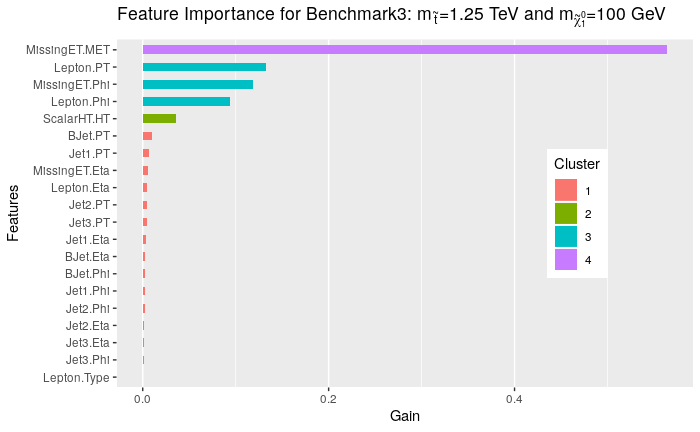
\includegraphics[width=\linewidth, keepaspectratio=true]{imp3.png}
    %\captionof{figure}{Feynman diagram of the leading order background process $pp \rightarrow t \Bar{t} \rightarrow b\Bar{b}l^{+}jj\cancel{\it{E}}_{T} $.}
    \label{fig:imp3}
  \end{minipage}
  \hfill
  \begin{minipage}[htbp]{0.45\textwidth}
    \centering
    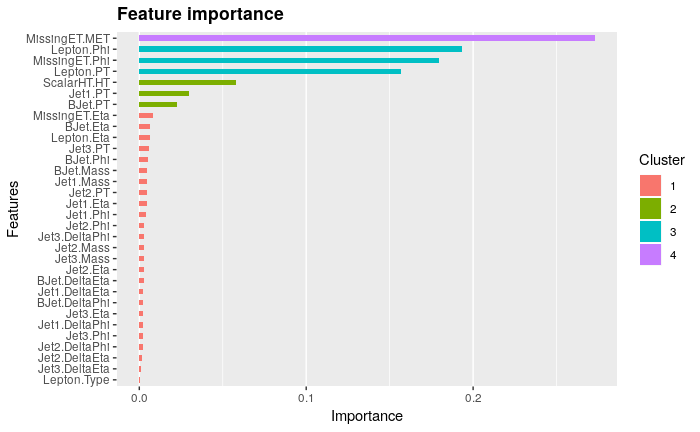
\includegraphics[width=\linewidth, keepaspectratio=true]{imp_in.png}
    %\captionof{figure}{Feynman diagram of the leading order signal process $ pp \rightarrow \Tilde{t}\Tilde{t^*} \rightarrow t \Bar{t} \chi^0_1\chi^0_1 \rightarrow b\Bar{b}l^{+}jj\cancel{\it{E}}_{T} $ where the final states are identical to that of the background in Figure \ref{fig:bkrdFeyn}.}
    \label{fig:imp_n}
  \end{minipage}
  \caption{The feature importance for all four benchmark points ordered from top-left to bottom-right. All four classifiers considers $\cancel{\it{E}}_{T}$ the most important feature, followed by the $\phi$ component of $\cancel{\it{E}}_{T}$ and the lepton as well as the lepton's $p_T$, not necessarily in this order. Furthermore the fifth most important variable is $H_T$ opposed to a particular jet's $p_T$. The clustering helps us to undestand the which variables were grouped together when considering a split. (??  Unsure about this explanation as I cannot find a good reference on the internet for it.)}
  \label{fig:imps}
\end{figure}

From the bar-plots shown in Figure \ref{fig:imps}, we notice that the algorithm had the highest contribution from the variable $\cancel{\it{E}}_{T}$ thus making it the most important. This is to be expected as we know that the neutralinos contribute to $\cancel{\it{E}}_{T}$ but also the SM neutrinos due to the highly energetic top quarks produced in our signal events. The next highest contributors were the $\phi$ components of $\cancel{\it{E}}_{T}$ and the lepton as well as its $p_T$, followed by the hadronic energy $H_T$. These five variables were consistently the top-five contributors to the algorithm and observing the grouping (noted as clusters in the legend), we can infer that the in particular, that the $\phi$ components of $\cancel{\it{E}}_{T}$ and the lepton have some sort of correlation with an occasional contribution from the lepton's $p_T$. We also observe that the $p_T$ of the $b$-jet and the remaining jet with highest $p_T$ (referred to as jet-1 henceforth) occasionally have slight contribution to the algorithm, with the remaining variables considered almost irrelevant consistently.
%-------------------------------------------------------------------------%
\section{Data Visualisation using \textit{tourr}}

In this section, I would like to show how data visualisation could be useful in helping understand new physics beyond the SM better. By creating a two-dimensional projection of the data entailing of higher dimensions (i.e. many variables), we can observe the distribution of data points in such a projection. The \textit{tourr} package from R \cite{tourr} is an ideal program for such a task, producing interesting results. The projected tour requires an index to minimize the distance between certain points in a dataset, in which we chose to utilize the \textit{alpha-hull} index. A corresponding basis is generated with each projection, and the algorithm will search through potentially more optimal projections through each iteration. NEED TO EXPLAIN ABOUT ALPHA INDEX A BIT AND SHOW SOME SPLOTS AND TALK ABOUT THE PHYSICS WE CAN INTERPRET FROM IT.


%  \begin{table}[htbp]
%        \centering
%        \begin{tabular}{c||c|c|c|c}
%        \toprule
%        &\multicolumn{1}{c|}{\bfseries Benchmark1}  &
%        \multicolumn{1}{c|}{\bfseries Benchmark2}  &
%        \multicolumn{1}{c|}{\bfseries Benchmark3} &
%        \multicolumn{1}{c}{\bfseries Benchmark4} \\
%        \midrule
        %----------------------------------%
%        \textbf{Metric} & Proportion & Proportion & Proportion & Proportion \\
%        \midrule
%        \rowcolor{gray!6} TP & $42.0 \%$ & $43.8 \%$ & $44.9 \%$ & $39.3 \%$ \\
%        TN & $49.4 \%$ & $49.5 \%$ & $49.4 \%$ & $49.5 \%$ \\
%        \rowcolor{gray!6} FP & $0.6 \%$ & $0.5 \%$ & $0.6 \%$ & $0.5 \%$\\
%      FN & $8.0 \%$ & $6.2 \%$ & $5.1 \%$ & $10.7 \%$ \\
%        \rowcolor{gray!6} Accuracy & $91.3 \pm 0.2 \%$ & $93.3 \pm 0.2 \%$ & $94.2 \pm 0.2 \%$ & $88.8 \pm 0.2 \%$ \\
%        \midrule
%        $b$ & $403$ & $368$ & $371$ & $382$ \\
%        \rowcolor{gray!6} $s$ & $2$ & $46$ & $11$ & $53$ \\
%        SBR & $0.5\%$ & $12.5\%$ & $3.0\%$ & $13.9\%$\\
%        \rowcolor{gray!6} AMS & $0.098$ & $2.32$ & $0.56$ & $2.62$ \\
%        \bottomrule
%        \end{tabular}
%        \caption*{Proportion of important values obtained in the four benchmark parameters.}
%    \end{table}


%-------------------------------------------------------------------------%
\chapter{Concluding Remarks}
%\section{Conclusion}
\vspace{-0.5cm}
In this project, we explored the simplified model of the top squark decays, namely the process: $pp \rightarrow \Tilde{t}\Tilde{t^*} \rightarrow t \Bar{t} \Tilde{\chi^0_1}\Tilde{\chi^0_1} \rightarrow b\Bar{b}jjl\cancel{\it{E}}_{T}$ by simulating this process through MadGraph, Pythia and Delphes, for four different mass parameters for the top squarks and neutralinos. Three were sitting just outside the exclusion curve (demarcated in black in Figure \ref{fig:limits}) and the other sitting well within the curve. \\

We used a machine learning algorithm known as xgboost to discriminate the signal and background events, followed by a simple statistical analysis using the approximate median significance (AMS). The three mass parameters outside the curve produce AMS values of 0.1, 0.31 and 0.6 suggesting that the background-only hypothesis for both discovery and upper limits is expected to be inconclusive. In contrast, the parameters from within the exclusion curve resulted in an AMS value of 2.8 associated with a relatively low SBR of 15.7\%, given that the integrated luminosity is 137 $\text{fb}^{-1}$. This is a high AMS value, and by using a smaller luminosity value at 35.9 $\text{fb}^{-1}$, we observe this to reduce to AMS=1.37 with the SBR remaining relatively low at 15.6\%. This shows that indeed, this parameter $m_{\Tilde{t}} = 750$ GeV and $m_{\Tilde{\chi}_1^0} = 1$ GeV is also excluded from searches. \\

We also turned to a high-dimensional data visualisation known as a guided tour to observe the patterns within the data as well as what qualities of the signal-like and background-like events made our classifiers perform poorly for such points. The most contributing variables were shown to be $\cancel{\it{E}}_{T}$ and the azimuthal component ($\phi$) of the $\cancel{\it{E}}_{T}$ and the charged leptons. The signal-like events showed a large spread in energy and angular dependence in most directions except for values closest to the $x$-direction orthogonal to the beam axis. The background-like events were distributed close to the $x$-direction orthogonal to the beam axis, that we can imagine the charged lepton and missing energy to have a narrow separation in the final states. This was further shown in a distribution plot for $\Delta \phi(\cancel{\it{E}}_{T},l)$ with a narrow distribution for the background events and broader distribution for the signal events. As expected, the difference in energy for the events remained the main contributor to differentiate signal and background. \\

In future, we can improve the methods in our analysis by incorporating the new $\Delta \phi(\cancel{\it{E}}_{T},l)$ variable, and other physically motivated variables seen in cut-based searches $\Delta \phi(\cancel{\it{E}}_{T},l)$. We can also perform simulations in MadGraph with Next-to-leading order (NLO) calculations instead of LO for more accurate kinematics. Furthermore, with the guided tour showing an important relationship that is $\Delta \phi(\cancel{\it{E}}_{T},l)$, we showed that data visualisation with a guided tour is an effective tool for data analysis, hence it is recommended for use in other searches as well.

\clearpage
%-------------------------------------------------------------------------%


%-------------------------------------------------------------------------%
%\newpage
\bibliographystyle{vancouver}
\bibliography{Thesis}

%-------------------------------------------------------------------------%


\end{document}
